\UseRawInputEncoding
%%%%%%%%%%%%%%%%%%%%%%%%%%%%%%%%%%%%%%%%%%%%%%%%%%%%%%%%%%%%%%%%%%%%%%%%%%%%%%%
%                       CARREGA DE LA CLASSE DE DOCUMENT                      %
%                                                                             %
% Les opcions admissibles son:                                                %
%      12pt / 11pt            (cos dels tipus de lletra; no feu servir 10pt)  %
%                                                                             %
% catalan/spanish/english     (llengua principal del treball)                 %
%                                                                             % 
% french/italian/german...    (si necessiteu fer servir alguna altra llengua) %
%                                                                             %
% listoffigures               (El document inclou un Index de figures)        %
% listoftables                (El document inclou un Index de taules)         %
% listofquadres               (El document inclou un Index de quadres)        %
% listofalgorithms            (El document inclou un Index d'algorismes)      %
%                                                                             %
%%%%%%%%%%%%%%%%%%%%%%%%%%%%%%%%%%%%%%%%%%%%%%%%%%%%%%%%%%%%%%%%%%%%%%%%%%%%%%%

\documentclass[11pt,spanish,listoffigures,listoftables]{tfgetsinf}

%%%%%%%%%%%%%%%%%%%%%%%%%%%%%%%%%%%%%%%%%%%%%%%%%%%%%%%%%%%%%%%%%%%%%%%%%%%%%%%
%                     CODIFICACIO DEL FITXER FONT                             %
%                                                                             %
%    windows fa servir normalment 'ansinew'                                   %
%    amb linux es possible que siga 'latin1' o 'latin9'                       %
%    Pero el mes recomanable es fer servir utf8 (unicode 8)                   %
%                                          (si el vostre editor ho permet)    % 
%%%%%%%%%%%%%%%%%%%%%%%%%%%%%%%%%%%%%%%%%%%%%%%%%%%%%%%%%%%%%%%%%%%%%%%%%%%%%%%

\usepackage[utf8]{inputenc}

%%%%%%%%%%%%%%%%%%%%%%%%%%%%%%%%%%%%%%%%%%%%%%%%%%%%%%%%%%%%%%%%%%%%%
% Para conseguir que la tabla de contenido no salga en rojo
%%%%%%%%%%%%%%%%%%%%%%%%%%%%%%%%%%%%%%%%%%%%%%%%%%%%%%%%%%%%%%%%%%%%%

\hypersetup{ colorlinks=true, linkcolor=black, urlcolor=cyan, }

%%%%%%%%%%%%%%%%%%%%%%%%%%%%%%%%%%%%%%%%%%%%%%%%%%%%%%%%%%%%%%%%%%%%%%%%%%%%%%%
%                        ALTRES PAQUETS I DEFINICIONS                         %
%                                                                             %
% Carregueu aci els paquets que necessiteu i declareu les comandes i entorns  %
%                                          (aquesta seccio pot ser buida)     %
%%%%%%%%%%%%%%%%%%%%%%%%%%%%%%%%%%%%%%%%%%%%%%%%%%%%%%%%%%%%%%%%%%%%%%%%%%%%%%%

\usepackage[T1]{fontenc}
\usepackage{listings}
\usepackage[most]{tcolorbox}
\usepackage{booktabs}
\usepackage{amssymb}
\usepackage{tabularx}
\usepackage{cleveref}
\usepackage{graphicx}  % Figuras en img/*.jpg (formato recomendado ETSINF)
\usepackage{placeins}  % \FloatBarrier — evita floats fuera de su sección
\usepackage{float}     % opción [H] si hace falta anclar una figura

\lstset{
    extendedchars=true,
    % Format: {input_char}{{output_latex}} length
    literate={á}{{\'a}}1 {é}{{\'e}}1 {í}{{\'i}}1 {ó}{{\'o}}1 {ú}{{\'u}}1
             {Á}{{\'A}}1 {É}{{\'E}}1 {Í}{{\'I}}1 {Ó}{{\'O}}1 {Ú}{{\'U}}1
             {ñ}{{\~n}}1 {Ñ}{{\~N}}1 {¿}{{\textquestiondown}}1 {¡}{{\textexclamdown}}1
             {—}{{--}}1 {–}{{-}}1
}

%%%%%%%%%%%%%%%%%%%%%%%%%%%%%%%%%%%%%%%%%%%%%%%%%%%%%%%%%%%%%%%%%%%%%%%%%%%%%%%
%                        DADES DEL TREBALL                                    %
%                                                                             %
% titol, alumne, tutor i curs academic                                        %
%%%%%%%%%%%%%%%%%%%%%%%%%%%%%%%%%%%%%%%%%%%%%%%%%%%%%%%%%%%%%%%%%%%%%%%%%%%%%%%

\title{Análisis comparativo de seguridad entre modelos de Defensa Perimetral y Zero Trust en infraestructuras contenerizadas}
\author{Pau Pérez Marco}
\tutor{Hector Marco Gisbert}
\curs{4º}

%%%%%%%%%%%%%%%%%%%%%%%%%%%%%%%%%%%%%%%%%%%%%%%%%%%%%%%%%%%%%%%%%%%%%%%%%%%%%%%
%                     PARAULES CLAU/PALABRAS CLAVE/KEY WORDS                  %
%                                                                             %
% Independentment de la llengua del treball, s'hi han d'incloure              %
% les paraules clau i el resum en els tres idiomes                            %
%%%%%%%%%%%%%%%%%%%%%%%%%%%%%%%%%%%%%%%%%%%%%%%%%%%%%%%%%%%%%%%%%%%%%%%%%%%%%%%

\keywords{} % Paraules clau 
         {Ciberseguridad, Zero Trust, Micro-segmentación, Contenedores, Post-explotación}      % Palabras clave
         {Cybersecurity, Zero Trust, Micro-segmentation, Containers, Post-exploitation}       % Key words

%%%%%%%%%%%%%%%%%%%%%%%%%%%%%%%%%%%%%%%%%%%%%%%%%%%%%%%%%%%%%%%%%%%%%%%%%%%%%%%
%                              INICI DEL DOCUMENT                             %
%%%%%%%%%%%%%%%%%%%%%%%%%%%%%%%%%%%%%%%%%%%%%%%%%%%%%%%%%%%%%%%%%%%%%%%%%%%%%%%

\begin{document}

%%%%%%%%%%%%%%%%%%%%%%%%%%%%%%%%%%%%%%%%%%%%%%%%%%%%%%%%%%%%%%%%%%%%%%%%%%%%%%%
%              RESUMS DEL TFG EN VALENCIA, CASTELLA I ANGLES                  %
%%%%%%%%%%%%%%%%%%%%%%%%%%%%%%%%%%%%%%%%%%%%%%%%%%%%%%%%%%%%%%%%%%%%%%%%%%%%%%%

\begin{abstract}[spanish]
Las nuevas arquitecturas basadas en microservicios y contenedores han servido para optimizar el despliegue de infraestructuras de red, pero frecuentemente, estos despliegues heredan configuraciones de red planas que amplían la superficie de ataque interno. En este contexto, las defensas perimetrales tradicionales resultan ineficaces cuando un atacante logra comprometer un servicio expuesto, facilitando la escalada de privilegios y el compromiso total del sistema. Este Trabajo de Fin de Grado presenta un análisis comparativo entre el modelo de seguridad perimetral tradicional y un modelo de arquitectura basada en principios Zero Trust mediante micro-segmentación. Para ello, se diseñan y despliegan dos infraestructuras funcionalmente idénticas. Ambas arquitecturas son sometidas a auditorías de seguridad focalizadas en escenarios de post-explotación y mediante la evaluación de métricas de contención y detección, el estudio cuantifica la eficacia de cada modelo de red. El trabajo busca demostrar que la implementación de una arquitectura Zero Trust bloquea eficazmente el movimiento lateral, mitiga el impacto de las intrusiones y resulta fundamental para garantizar la resiliencia en redes corporativas modernas.
\end{abstract}

\begin{abstract}[english]
New microservices and container-based architectures have optimized the deployment of network infrastructures; however, these deployments frequently inherit flat network configurations that expand the internal attack surface. In this context, traditional perimeter defenses become ineffective once an attacker manages to compromise an exposed service, facilitating privilege escalation and the total compromise of the system. This Bachelor's Thesis presents a comparative analysis between the traditional perimeter security model and an architecture model based on Zero Trust principles through micro-segmentation. To this end, two functionally identical infrastructures are designed and deployed. Both architectures are subjected to security audits focused on post-exploitation scenarios. By evaluating containment and detection metrics, the study quantifies the effectiveness of each network model. The work seeks to demonstrate that the implementation of a Zero Trust architecture effectively blocks lateral movement, mitigates the impact of intrusions, and is fundamental to ensuring resilience in modern corporate networks.
\end{abstract}

%%%%%%%%%%%%%%%%%%%%%%%%%%%%%%%%%%%%%%%%%%%%%%%%%%%%%%%%%%%%%%%%%%%%%%%%%%%%%%%
%                              CONTINGUT DEL TREBALL                          %
%%%%%%%%%%%%%%%%%%%%%%%%%%%%%%%%%%%%%%%%%%%%%%%%%%%%%%%%%%%%%%%%%%%%%%%%%%%%%%%

\mainmatter

%%%%%%%%%%%%%%%%%%%%%%%%%%%%%%%%%%%%%%%%%%%%%%%%%%%%%%%%%%%%%%%%%%%%%%%%%%%%%%%
% ÍNDICE DE MARCADORES PENDIENTES — buscar en el archivo: [PENDIENTE:
% Pasada CITAR:    RESUELTA — \cite{} en cuerpo + entradas en thebibliography; herramientas y webs como \footnote{}
% Pasada REVISAR:  RESUELTA — decisiones aplicadas (tabla Wazuh en cap. 5; figura Wazuh única en sec:4.3.4)
% Pasada COMPLETAR: RESUELTA — metadatos de fuentes verificados (TFG/TFM, NIST, Forrester, IBM, Verizon, MITRE)
% Pasada FIG:      COMPLETADA — 32 esqueletos en img/*.jpg (véase img/README.md)
% Pasada PENDIENTE: RESUELTA — anexos completos (protocolo, configuración, despliegue/captura, Wazuh, código) y glosario (acrónimos + términos)
%%%%%%%%%%%%%%%%%%%%%%%%%%%%%%%%%%%%%%%%%%%%%%%%%%%%%%%%%%%%%%%%%%%%%%%%%%%%%%%

%%%%%%%%%%%%%%%%%%%%%%%%%%%%%%%%%%%%%%%%%%%%%%%%%%%%%%%%%%%%%%%%%%%%%%%%%%%%%%%
%                                  INTRODUCCIO                                %
%%%%%%%%%%%%%%%%%%%%%%%%%%%%%%%%%%%%%%%%%%%%%%%%%%%%%%%%%%%%%%%%%%%%%%%%%%%%%%%

\chapter{Introducci\'on}
    \section{Motivaci\'on}
    Una brecha de seguridad reciente expuso los datos personales de cerca de 300.000 clientes de Endesa, una de las mayores compañías energéticas de España\footnote{Higuera, A. \textit{Hackeo a Endesa: el autor asegura que ha publicado datos de 300.000 clientes y que solo son ``una muestra''}. 20minutos, 30 de enero de 2026. \url{https://www.20minutos.es/tecnologia/ciberseguridad/datos-hackeo-endesa-300000-clientes_6926723_0.html} (consultado el 30 de enero de 2026).}. Lejos de ser un caso aislado, incidentes como este se han vuelto frecuentes y ponen el foco sobre una preocupante realidad: el coste económico de la ciberdelincuencia aumenta año tras año a escala global \cite{costdatabreach}. Para cualquier organización, una intrusión ha dejado de ser un suceso excepcional para convertirse en un riesgo que conviene asumir y prevenir.

    Al mismo tiempo, la manera de construir y desplegar software ha cambiado. Las arquitecturas basadas en microservicios y contenedores se han generalizado porque agilizan el despliegue y el escalado de las aplicaciones. Esa comodidad, sin embargo, tiene una contrapartida de seguridad: muchos despliegues heredan configuraciones de red planas, en las que los servicios internos confían entre sí por el simple hecho de compartir la misma red. El resultado es una superficie de ataque interior que apenas está controlada.
    
    El modelo de seguridad perimetral, sobre el que se ha apoyado tradicionalmente la protección de las redes corporativas, encaja mal con este escenario. Su planteamiento protege la frontera entre la red interna y el exterior, pero presupone que todo lo que sucede dentro del perímetro es de confianza. Cuando un atacante compromete un único servicio expuesto, esa confianza implícita se vuelve en su contra: puede desplazarse lateralmente, alcanzar servicios internos o bases de datos y extraer información sin volver a cruzar ninguna frontera vigilada. El modelo Zero Trust parte de la premisa opuesta y no concede confianza por defecto a ningún componente, ni siquiera a los que ya operan dentro de la red.
    
    Este contraste entre lo que el perímetro promete y lo que realmente contiene una vez producida la intrusión es lo que motiva el presente trabajo. Más que defender un modelo frente a otro en el plano teórico, nos proponemos medir, en condiciones reproducibles, cuánto reduce el impacto de un ataque interno una arquitectura Zero Trust frente a un despliegue perimetral equivalente.
    
    \section{Objetivos}
    \label{sec:1.2}
        \subsection{Pregunta de investigación}
        El trabajo se articula en torno a una única pregunta de investigación, que orienta tanto el diseño de la solución como las pruebas realizadas:

        \begin{tcolorbox}[
            enhanced,
            frame hidden,
            borderline west={3pt}{0pt}{gray!70!black},
            sharp corners
        ]
            ¿En qué medida aplicar la metodología Zero Trust reduce el impacto de ataques post-explotación frente a un modelo perimetral, y cómo lo hace esto superior?
        \end{tcolorbox}


        \subsection{Hipótesis}
        Como respuesta a esa pregunta partimos de la siguiente hipótesis: \emph{los mecanismos propios de una arquitectura Zero Trust: la microsegmentación de la red y la identidad de servicio mediante mTLS (Mutual TLS), reducen de forma apreciable la profundidad del compromiso, el volumen de datos exfiltrados y en general, la capacidad del atacante de hacer el máximo daño posible, en comparación con un modelo perimetral funcionalmente equivalente.} El estudio se concibe para contrastar esta hipótesis con datos medibles.

        \subsection{Objetivo principal}
        El objetivo principal de este trabajo es medir cuánto reduce el impacto de un ataque interno una arquitectura Zero Trust. Para ello, se diseñan y despliegan dos infraestructuras funcionalmente idénticas y ambas son sometidas a auditorías de seguridad basadas en escenarios de post-explotación para que, mediante la evaluación de métricas de contención y detección, el estudio pueda cuantificar la eficacia de cada modelo de red.

        \subsection{Objetivos específicos}
        De este objetivo principal se derivan cuatro objetivos específicos:
        \begin{itemize}
            \item Diseñar y desplegar dos infraestructuras funcionalmente idénticas sobre Docker.
            \item Definir y medir un conjunto de métricas de contención y detección comparables entre ambos escenarios.
            \item Ejecutar pruebas de post-explotación reproducibles: movimiento lateral, exfiltración e interceptación de tráfico interno en los dos escenarios.
            \item Instalar un sistema de detección (observabilidad) como capa adicional de seguridad.
        \end{itemize}

    \section{Impacto esperado}
    Los resultados de este trabajo aspiran a ser útiles para dos perfiles:
    \begin{enumerate}
        \item Para los equipos de plataforma y de seguridad operativa (DevSecOps). Este trabajo ofrece un criterio cuantitativo con el que justificar la inversión en microsegmentación e identidad de servicio, más allá de la recomendación genérica de adoptar Zero Trust. 
        \item Para las organizaciones que mantienen despliegues contenerizados heredados, aportan evidencia del riesgo real al que se exponen tras una intrusión y del grado de contención que pueden alcanzar con controles asumibles.
    \end{enumerate}
    
    En un plano más amplio, el trabajo se relaciona con los Objetivos de Desarrollo Sostenible, en particular con el ODS 9 (\emph{Industria, Innovación e Infraestructura}), por su contribución a infraestructuras digitales más resilientes, y con el ODS 16 (\emph{Paz, Justicia e Instituciones sólidas}), por la reducción del impacto de la ciberdelincuencia. 
    
    \section{Metodología}
    El trabajo sigue un enfoque experimental. Diseñamos dos prototipos funcionalmente idénticos y los desplegamos en un laboratorio basado en Docker, definido como infraestructura como código (IaC) para que cada escenario pueda levantarse de forma reproducible. Sobre ambos ejecutamos la misma cadena de ataque y los sometemos a las mismas pruebas, y a su vez, capturamos de manera estructurada las evidencias generadas para su análisis cuantitativo posterior.

    La comparación solo es válida si los dos escenarios se miden en las mismas condiciones. Por ese motivo empleamos el mismo atacante simulado y una ventana de medición común, que comienza en el instante en que el atacante dispone de ejecución remota en el servicio web. Así, todo lo que se mide ocurre a partir de un punto de partida equivalente en ambos escenarios. El protocolo operativo detallado se describe en el anexo \ref{anexo:protocolo_ejecucion}.  
    
    \section{Estructura de la mem\`oria}
    El resto de la memoria se organiza como sigue:
    \begin{itemize}
        \item El capítulo 2 revisa el estado del arte: el modelo perimetral y sus limitaciones, los principios de Zero Trust y la microsegmentación, las amenazas en fase de post-explotación y los trabajos relacionados, para situar la aportación de este trabajo.
        \item El capítulo 3 analiza el problema, formaliza el modelo de amenazas, fija los requisitos y define las métricas con las que se evalúan ambos escenarios.
        \item El capítulo 4 presenta el diseño de las dos arquitecturas comparadas y justifica las decisiones tecnológicas adoptadas.
        \item El capítulo 5 describe el desarrollo y la implantación del laboratorio, incluidos los problemas de integración encontrados.
        \item El capítulo 6 expone la metodología de pruebas y los resultados de cada escenario, junto con la comparativa final entre ambos.
        \item Por último, el capítulo 7 recoge las conclusiones, las limitaciones del trabajo, las líneas de trabajo futuro y la relación con los estudios cursados y los ODS.
    \end{itemize}

    La memoria se completa con la bibliografía y con una serie de anexos que recogen el código fuente de la aplicación (\cref{anexo:codigo_aplicacion}), las configuraciones extensas de ambos escenarios (ficheros de despliegue, configuración de mTLS y generación de certificados, \cref{anexo:configuracion}), las reglas de detección y los scripts de captura de evidencias (\cref{anexo:scripts_captura}). Asimismo, al final se incluye un glosario de términos y acrónimos (\cref{anexo:glosario}) que conviene consultar ante cualquier duda sobre la terminología específica utilizada a lo largo del texto.


%\section{Notes bibliografiques} %%%%% Opcional

%%%%%%%%%%%%%%%%%%%%%%%%%%%%%%%%%%%%%%%%%%%%%%%%%%%%%%%%%%%%%%%%%%%%%%%%%%%%%%%
%                                CAPÍTULOS                                    %
%%%%%%%%%%%%%%%%%%%%%%%%%%%%%%%%%%%%%%%%%%%%%%%%%%%%%%%%%%%%%%%%%%%%%%%%%%%%%%%

\chapter{Estado del arte}
    \section{El modelo de seguridad perimetral y sus limitaciones}
    \label{sec:2.1}
    La seguridad perimetral ha constituido durante décadas el paradigma predominante para la protección de redes corporativas. Este modelo utiliza una frontera entre una red interna y la externa como elemento de seguridad. Para ello, utiliza mecanismos como firewalls, filtros y controles de acceso. A su vez, asume que los usuarios y dispositivos ubicados dentro del perímetro, dentro de la red, son entidades confiables. 
    
    Históricamente, este enfoque resultó eficaz en tiempos en los que las organizaciones tenían infraestructuras centralizadas y límites de red claramente definidos, y donde la principal amenaza procedía de actores externos \cite{perimetro}.
    
    Sin embargo, con el paso de los años, se han observado limitaciones significativas cuando un atacante consigue superar los controles perimetrales iniciales. La confianza otorgada a los sistemas internos facilita en gran medida las actividades de post-explotación, incluyendo el movimiento lateral, la escalada de privilegios y el acceso no autorizado a recursos críticos.
    
    Asimismo, la evidencia reciente refuerza estas limitaciones: en 2025 se identificó el abuso de credenciales y la explotación de vulnerabilidades entre los principales vectores de acceso y explotación inicial, mientras que casi un tercio de las brechas tuvo origen interno \cite{breaches2025}.  Estos resultados evidencian que la protección exclusiva del perímetro resulta insuficiente frente a las amenazas modernas.

    \section{El modelo Zero Trust}
    \label{sec:2.2}
    El modelo Zero Trust apareció oficialmente en 2010, cuando John Kindervag, entonces analista de Forrester Research, lo formuló como respuesta a las limitaciones de los enfoques de seguridad basados en la confianza implícita dentro de las redes corporativas \cite{kindervag2010}. Su propuesta se fundamenta en la premisa de que ningún usuario, dispositivo o sistema debe considerarse confiable por defecto, dando origen al principio \emph{"never trust, always verify"}.
     
    Con el tiempo, este planteamiento evolucionó hasta convertirse en un marco de referencia. La publicación NIST SP 800-207 \cite{nist800207} consolidó esta evolución al definir una arquitectura Zero Trust basada en la verificación continua de identidades, la autorización dinámica, el acceso de mínimo privilegio y la evaluación contextual de usuarios, dispositivos y recursos. Debido al impacto que tuvo, la microsegmentación y la protección centrada en los recursos se establecieron como mecanismos esenciales para reducir la superficie de ataque.
    
    BeyondCorp, desarrollada por Google en 2014 \cite{beyondcorp}, fue la primera iniciativa en trasladar los principios de Zero Trust a una infraestructura empresarial de gran escala, sustituyendo la confianza basada en la ubicación de red por reglas de acceso fundamentadas en la identidad del usuario y el estado de los dispositivos, esto contribuyó significativamente a la difusión del modelo y a la demostración de su viabilidad, lo que concluyó en su consolidación en la industria y la comunidad académica.

        \subsection{Microsegmentación en entornos contenerizados}
        \label{sec:2.2.1}
        Los principios de Zero Trust consisten en gran medida en técnicas de microsegmentación, cuyo objetivo es eliminar la confianza entre recursos internos y establecer controles de acceso sobre las comunicaciones de red. La microsegmentación permite restringir el acceso entre servicios y limitar la exposición de recursos, de esta forma se reduce la superficie de ataque y dificulta el movimiento lateral de un atacante tras una intrusión.
        
        En entornos contenerizados, como aquellos gestionados por Kubernetes (común en redes corporativas modernas), esta estrategia suele implementarse mediante la creación de redes virtuales independientes que agrupan servicios según su función. Para ayudar a este fin, Docker proporciona mecanismos de aislamiento de red que permiten definir explícitamente qué contenedores pueden comunicarse entre sí. Además de esto, las arquitecturas modernas incorporan mecanismos de identidad de servicio y autenticación mutua mediante certificados digitales para reforzar la confianza entre componentes distribuidos. A mayor escala, se utilizan Network Policies, que permiten controlar el tráfico de ingreso y salida entre pods mediante reglas declarativas y etiquetas.

    \section{Amenazas en entornos post-explotación de contenedores}
    \label{sec:2.3}
    A pesar de los mecanismos de protección proporcionados, la obtención de ejecución remota de código (RCE) dentro de una aplicación sigue constituyendo un punto de partida relevante para actividades de post-explotación. Un contenedor comprometido puede convertirse en una plataforma desde la que explorar recursos internos, acceder a servicios auxiliares y obtener información sensible dentro del entorno.
    
    Diversos marcos de análisis de amenazas, como MITRE ATT\&CK for Containers y Kubernetes Threat Matrix \cite{mitrecontainers}, documentan técnicas de reconocimiento interno, abuso de credenciales y movimiento lateral utilizadas para ampliar progresivamente el alcance del compromiso. Asimismo, la presencia de secretos en variables de entorno, archivos de configuración, volúmenes compartidos o mecanismos de almacenamiento insuficientemente protegidos puede facilitar la exfiltración de credenciales y datos sensibles. Otro riesgo significativo está relacionado con las comunicaciones este-oeste entre servicios: cuando el tráfico interno no está cifrado, un atacante con presencia en el entorno puede capturar credenciales o información confidencial en tránsito.
    
    Estas amenazas adquieren especial relevancia en entornos cloud-native debido al elevado número de interacciones entre servicios y a la creciente complejidad de las dependencias internas, lo que incrementa las oportunidades de expansión del atacante una vez superada la fase inicial de acceso.

    \section{Trabajos relacionados}
    \label{sec:2.4}
    Para la realización de este trabajo, se han estudiado algunos trabajos similares dentro de este mismo ámbito para entender el contexto de la situación académica:
    \begin{itemize}
        \item Jiménez 2025 TFG UPM — implementación ZT laboratorio \cite{jimenez2025} diseña e implementa un entorno Zero Trust híbrido simulado con identidad federada, segmentación mediante firewall y aplicación web en Flask. Valida la autenticación y las políticas de acceso de forma funcional, pero no ejecuta una cadena adversarial post-explotación ni contrasta el resultado con un escenario perimetral de referencia.
        \item Pérez TFG G6508 — Zero Trust como concepto \cite{perezg6508} profundiza en el marco teórico, modelos frente a arquitecturas, visión de fabricantes, normalización NIST— y plantea un despliegue ZTNA a escala empresarial, sin experimento que cuantifique el impacto de un atacante.
        \item Torregrosa 2025 TFG UPV — NAC y acceso corporativo \cite{torregrosa2025}, aborda el acceso local mediante NAC y segmentación dinámica alineada con Zero Trust, centrado en quién entra a la red corporativa, no en qué puede hacer un servicio comprometido en comunicaciones este-oeste entre microservicios. 
        \item Vico 2025 TFM UPV — SIEM Wazuh Suricata \cite{vico2025}, integra Wazuh, Suricata y un SIEM corporativo para centralizar la detección. Su aportación está en el pipeline de observabilidad y los casos de uso de alertas, no en comparar arquitecturas de red ni en medir la contención del movimiento lateral tras una ejecución remota.
    \end{itemize}
    
    \section{Crítica al estado del arte}
    La revisión de los apartados anteriores muestra, por un lado, que las limitaciones del modelo perimetral frente a las amenazas posteriores al compromiso están ampliamente documentadas (\cref{sec:2.1}). 
    
    Por otro lado, que los mecanismos asociados a Zero Trust (microsegmentación, identidad de servicio y autenticación mutua) cuentan con viabilidad demostrada, tanto en la estandarización de NIST SP 800-207 como en implementaciones a gran escala como BeyondCorp (\cref{sec:2.2}, \cref{sec:2.2.1}).
    
    Y finalmente, que las técnicas de post-explotación en entornos contenerizados están catalogadas en marcos como MITRE ATT\&CK for Containers y la Kubernetes Threat Matrix (\cref{sec:2.3}). 
    
    Sin embargo, estos tres cuerpos rara vez se articulan entre sí, echamos en falta una fuente que enfoque directamente la idea de por qué Zero Trust debería ser el estándar a la hora de la implementación de redes, con métricas que cuantifiquen en qué medidas esos mecanismos contienen a un atacante.
    
    A su vez, en los últimos años han proliferado trabajos académicos que abordan Zero Trust desde ángulos distintos: 
    \begin{itemize}
        \item implementación en laboratorio
        \item análisis conceptual
        \item control de acceso a la red corporativa
        \item observabilidad centralizada
    \end{itemize}
    
    Ahora bien, al revisar la literatura y los trabajos de fin de grado o máster más cercanos al ámbito de este proyecto, se observa un patrón recurrente: demuestran la viabilidad de un enfoque concreto, pero rara vez miden de forma cuantitativa qué ocurre en la práctica, después de un compromiso inicial. La evidencia que compara el modelo perimetral y Zero Trust sigue siendo escasa.
    
    \section{Propuesta}
    Este trabajo se sitúa en este hueco. Su aportación no es una tecnología nueva, es la combinación original y la medición controlada de mecanismos ya existentes. Para ello, proponemos recoger los principales aprendizajes de las fuentes técnicas y trabajos académicos con el fin de realizar un experimento controlado en el que enlazar las limitaciones del perímetro (\cref{sec:2.1}), las amenazas post-explotación (\cref{sec:2.3}) y la mejora gracias a la implementación de Zero Trust desarrollada en los capítulos siguientes.

%%%%%%%%%%%%%%%%%%%%%%%%%%%%%%%%%%%%%%%%%%%%%%%%%%%%%%%%%%%%%

\chapter{Análisis del problema}
 
    \section{Descripción del problema}
    Las infraestructuras basadas en microservicios y contenedores facilitan el despliegue, pero a menudo heredan, por facilidad o simplicidad, configuraciones de red en las que, una vez comprometido un servicio expuesto al exterior, el atacante tiene libre acceso al resto de la red. Ese patrón reproduce la limitación del modelo perimetral que ya hemos analizado en \cref{sec:2.1} y las amenazas post-explotación descritas en \cref{sec:2.3}: el perímetro protege la entrada, no lo que ocurre después.
    
    La comparativa entre un escenario perimetral de referencia y un escenario Zero Trust es el método experimental con el que medimos esa reducción. En las secciones siguientes acotamos el modelo de amenazas, traducimos ese marco en requisitos verificables y definimos las métricas con las que cuantificaremos el impacto en el capítulo de pruebas.
    
    
    \section{Modelo de amenazas}
    \label{sec:3.2}
    El análisis del problema se centra en la fase post-explotación: asumimos que el atacante ya dispone de RCE en el servicio web y medimos qué puede hacer a partir de ese punto dentro de la red de contenedores. Este acotamiento delimita el experimento frente a vectores de acceso inicial o ataques contra el host físico, los cuales quedan fuera del alcance de medición.

    Los apartados \cref{sec:3.2.1} a \cref{sec:3.2.5} desarrollan las cinco dimensiones del modelo de amenazas que estructuran el resto de la memoria.
    
        \subsection{Asunciones sobre el atacante}
        \label{sec:3.2.1}
        Consideramos un atacante externo y no privilegiado que ha explotado una vulnerabilidad en el servicio web y obtiene ejecución de código remota en el contenedor de la aplicación. No dispone de acceso físico al equipo anfitrión ni de credenciales de administración de la red corporativa. 

        A partir de una reverse shell en \texttt{webapp} comienza la ventana de estudio: todo lo que se mide ocurre con el mismo nivel de privilegio dentro del namespace del contenedor comprometido.

        \subsection{Activos a proteger}
        \label{sec:3.2.2}
        Los activos prioritarios son: 
            \begin{enumerate}
                \item La base de datos PostgreSQL, que almacena los registros de empleados y las credenciales asociadas al entorno de prueba
                \item El backend de la aplicación, que concentra el código de la API interna y las variables de entorno sensibles (incluidas las credenciales de acceso a la base de datos).
            \end{enumerate}
            Un movimiento lateral exitoso desde \texttt{webapp} comprometida puede alcanzar esos activos sin cruzar de nuevo el perímetro exterior, por eso el estudio evalúa controles que limiten ese alcance.
            
        \subsection{Superficie de estudio}
        \label{sec:3.2.3}
        La superficie bajo análisis es la red interna de contenedores Docker y las comunicaciones este-oeste entre servicios: el flujo entre la aplicación web y el backend, y el flujo entre el backend y la base de datos. 

        No evaluamos el host Windows ni la capa de orquestación fuera del experimento, el foco son los controles que cada arquitectura aplica entre contenedores una vez el atacante opera desde \texttt{webapp}.
        
        \subsection{Amenazas en alcance}
        \label{sec:3.2.4}
        Dentro de ese marco consideramos tres amenazas principales:

        Primero, el \textbf{movimiento lateral}: uso de la posición en \texttt{webapp} para alcanzar el backend o la base de datos sin pasar por el único punto de entrada externo para acceder a otro contenedor.
        
        Segundo, la \textbf{interceptación del tráfico interno} entre servicios, en particular cuando las peticiones viajan en texto claro y pueden capturarse desde el contenedor comprometido. 
        
        Tercero, la \textbf{exfiltración de credenciales y datos almacenados}, incluido el volcado de tablas de la base de datos.
        
        En las pruebas materializamos esas amenazas mediante cuatro hitos post-explotación comunes (\cref{sec:4.2.3}): 
        \begin{enumerate}
            \item Exfiltración de credenciales del entorno del contenedor
            \item Escaneo de la red interna
            \item Acceso al backend
            \item Volcado de la base de datos
        \end{enumerate}
        Esos hitos son el denominador comparativo entre el escenario perimetral y el escenario Zero Trust.
        
        \subsection{Amenazas fuera del alcance}
        \label{sec:3.2.5}
        Quedan explícitamente fuera del alcance:
        \begin{enumerate}
            \item La ingeniería social y el phishing
            \item La seguridad física del dispositivo donde se hospedan las redes
            \item Las vulnerabilidades del kernel del sistema operativo subyacente
            \item Los ataques de denegación de servicio
            \item Cualquier vector cuya mitigación no depende directamente de la microsegmentación, la identidad de servicio o la detección host-based que implementamos en el escenario Zero Trust.
        \end{enumerate}
        Esta delimitación permite centrar el diseño y las pruebas en controles comparables entre arquitecturas sin dispersar el alcance del TFG.

    \section{Especificación de requisitos}
        \subsection{Requisitos funcionales}
        \label{sec:3.3.1}
        
        \begin{table}[ht]
          \centering
          \label{tab:requisitos-funcionales}
          \begin{tabular}{p{2.8cm} p{10cm}}
            \textbf{ID} & \textbf{Requisito} \\
            \midrule
            Requisito-F 1 & El sistema debe reproducir una cadena de acceso inicial reproducible hasta RCE en \texttt{webapp}. \\
            \midrule
            Requisito-F 2 & El sistema debe medir los 6 indicadores (G1--G3, E1--E3) de forma comparable entre Escenario A y B. \\
            \midrule
            Requisito-F 3 & El Escenario B debe bloquear o detectar los 4 hitos post-RCE del Escenario A. \\
            \midrule
            Requisito-F 4 & Las evidencias de cada escenario deben ser reproducibles y verificables (logs, capturas de tráfico, etc.). \\
            \bottomrule
          \end{tabular}
          \caption{Requisitos funcionales.}
        \end{table}
        
        Los requisitos funcionales traducen el modelo de amenazas y la pregunta de investigación en criterios que se deben cumplir:
        \begin{itemize}
            \item \textbf{Requisito-F 1} exige un acceso inicial reproducible hasta ejecución remota en `webapp`, de modo que el instante de inicio de la ventana post-explotación sea comparable en ambos escenarios.
            \item \textbf{Requisito-F 2} impone que los seis indicadores definidos en \cref{sec:3.4} se midan con el mismo protocolo de ataque una vez obtenida la reverse shell.
            \item \textbf{Requisito-F 3} vincula el escenario Zero Trust con el baseline perimetral: los cuatro hitos post-RCE alcanzables en el escenario A deben quedar bloqueados o, como mínimo, detectados en el escenario B.
            \item \textbf{Requisito-F 4} garantiza trazabilidad académica mediante logs, capturas de tráfico y artefactos de sesión que respalden cada valor reportado en el capítulo de resultados.
        \end{itemize}
        
        \subsection{Requisitos no funcionales}
        
        \begin{table}[ht]
          \centering
          \label{tab:requisitos-no-funcionales}
          \begin{tabular}{p{2.8cm} p{10cm}}
            \textbf{ID} & \textbf{Requisito} \\
            \midrule
            Requisito-NF 1 & Despliegue automatizado mediante \texttt{docker compose up} en un solo comando. \\
            \midrule
            Requisito-NF 2 & El entorno debe estar adaptado para ejecutarse en hardware de escritorio (sin infraestructura cloud). \\
            \midrule
            Requisito-NF 3 & Las capturas de evidencia deben almacenarse de forma estructurada y reproducible. \\
            \midrule
            Requisito-NF 4 & El código de infraestructura debe ser mantenible. \\
            \bottomrule
          \end{tabular}
          \caption{Requisitos no funcionales.}
        \end{table}
        
        Los requisitos no funcionales aseguran que el experimento sea repetible y suponen mejoras de calidad de vida para facilitar las pruebas:
        \begin{itemize}
            \item \textbf{Requisito-NF 1:} cada escenario se levanta con un único comando.
            \item \textbf{Requisito-NF 2:} acota el laboratorio a una estación de trabajo con Docker Desktop, sin depender de servicios cloud, lo que hace viable la réplica del estudio en condiciones académicas.
            \item \textbf{Requisito-NF 3:} exige que cada sesión de prueba deje una carpeta estructurada de evidencias.
            \item \textbf{Requisito-NF 4:} el código debe ser mantenible (compose legible, servicios separados, etc.)
        \end{itemize}
        En conjunto, estos requisitos se concretan en el diseño comparativo del \cref{sec:4} y se verifican en las sesiones documentadas en el \cref{sec:6}.
        
    \section{Definición de métricas}
    \label{sec:3.4}
    
    \begin{table}[ht]
      \centering
      \label{tab:kpi-definicion}
      \footnotesize
      \begin{tabularx}{\textwidth}{@{}l l X X@{}}
        \textbf{Código} & \textbf{Nombre} & \textbf{Definición} & \textbf{Operacionalización} \\
        \midrule
        G1 & Tiempo de detección & Tiempo desde inicio de medición hasta la primera alerta activa de seguridad. & Tupla \texttt{(mecanismo\_existe, segundos | $\infty$)}. \\
        \midrule
        G2 & Profundidad del ataque & Número de nodos o servicios internos a los que el atacante alcanza. & Conteo de servicios  \\
        \midrule
        G3 & Bloqueo de comandos desde reverse shell & Porcentaje de hitos post-RCE en los que un control impide o frustra la acción del atacante. & Tupla \texttt{(mecanismo\_existe, \%)}. Evaluación sobre los cuatro hitos de \cref{sec:3.2.4}. \\
        \midrule
        E1 & Superficie interna visible & Servicios y puertos internos descubiertos o alcanzables desde \texttt{webapp} tras RCE. & Recuento de servicios visibles en escaneo interno desde el contenedor comprometido. \\
        \midrule
        E2 & Volumen de datos exfiltrados & Cantidad y naturaleza de la información extraída en la ventana post-explotación. & Registros, credenciales y bytes exfiltrados \\
        \midrule
        E3 & Integridad del tráfico interno & Grado de protección de las comunicaciones este-oeste entre servicios. & Clasificación: tráfico en texto claro observable frente a TLS o conexión rechazada. \\
        \bottomrule
      \end{tabularx}
      \caption{Indicadores de evaluación y su operacionalización.}
    \end{table}
    
    Fijamos el instante de inicio de registro de evidencias en el momento en que la reverse shell en `webapp` queda operativa bajo control del atacante (RCE). A partir de ese instante medimos los seis indicadores de la tabla anterior.

    Para el tiempo de detección y el bloqueo de comandos desde reverse shell empleamos una tupla \texttt{(mecanismo\_existe, valor)}. En el escenario A no hay SIEM por diseño, ya que es lo que se asume de una configuración de red heredada y sin modificar, la tupla registra la ausencia del mecanismo.
    
    Los cuatro hitos post-explotación, numerados en \cref{sec:3.2.4}, alimentan sobre todo los indicadores de bloqueo, superficie visible y volumen exfiltrado. La integridad del tráfico se evalúa con captura de las comunicaciones entre \texttt{webapp} y \texttt{backend} durante el intento de movimiento lateral. Los valores obtenidos en cada escenario y el análisis comparativo se recogen en \cref{sec:6.4}.
    
%%%%%%%%%%%%%%%%%%%%%%%%%%%%%%%%%%%%%%%%%%%%%%%%%%%%%%%%%%%%%

\chapter{Diseño de la solución}
\label{sec:4}
El capítulo anterior ha fijado el marco experimental y, en este capítulo, traducimos ese análisis en decisiones de arquitectura concretas. Diseñamos el stack Docker que sirve la aplicación web y aplicamos distintas metodologías para crear los modelos de red deseados.

    \section{Arquitectura distribuida}
    Para el desarrollo de nuestra red, debemos diseñar una aplicación formada por microservicios que la componga.

        \subsection{Visión general del sistema}
        Como el objetivo del trabajo está centrado en la comparación a nivel de red, entre modelos, y cómo cada uno produce resultados diferentes, vamos a simplificar los flujos y la implementación de dicha aplicación web.

        Separamos la app web en 3 capas: Presentación, Lógica y Datos, cada capa se encuentra compuesta por un microservicio (contenedor):
        \begin{itemize}
            \item \textbf{webapp:} Frontal del sistema, un portal web con panel de administración.
            \item \textbf{backend:} con API interna de empleados que recibe peticiones del frontal.
            \item \textbf{DB (DataBase):} Base de datos PostgreSQL para almacenar información.
        \end{itemize}

        \begin{figure}[ht]
            \centering
            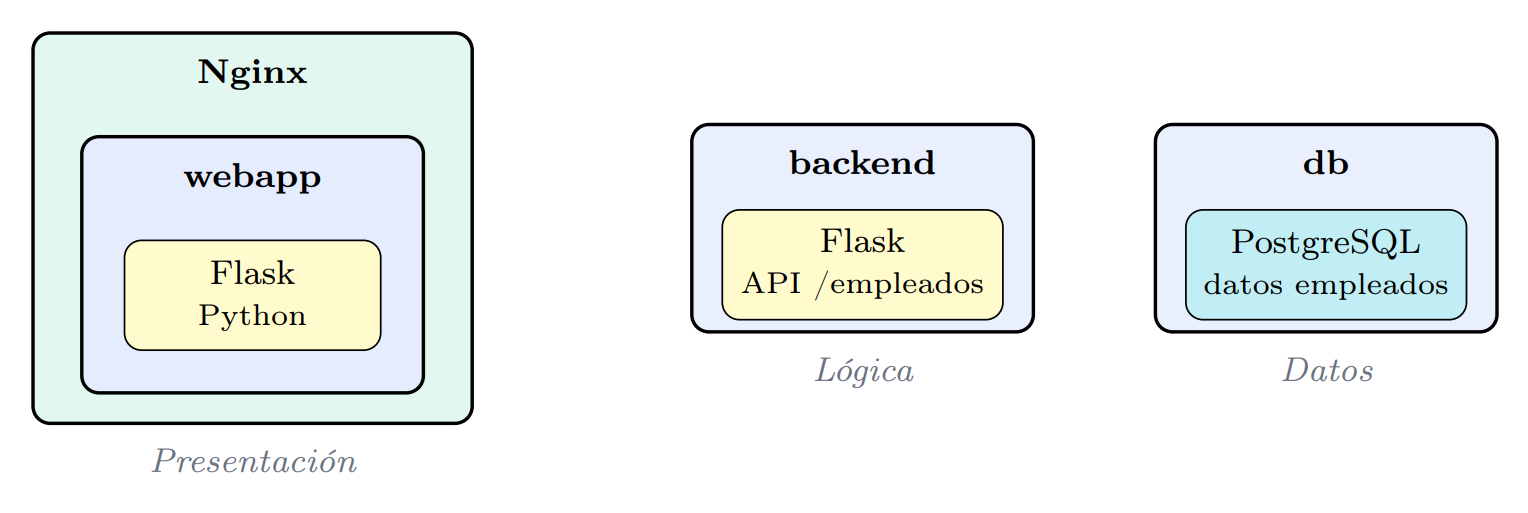
\includegraphics[width=0.9\linewidth]{img/cap04-arquitectura-microservicios.jpg}
            \caption{Arquitectura de microservicios: nginx sirve \texttt{webapp} (Flask), que consume la API de \texttt{backend} (Flask) y la base de datos PostgreSQL.}
            \label{fig:arquitectura-microservicios}
        \end{figure}

        La aplicación es funcionalmente idéntica en ambos escenarios, lo que cambia es el modelo de red.

        \subsubsection{Flujos detallados}
        \label{sec:4.1.1}
        Los flujos de la aplicación son deliberadamente simples, por lo que hemos mencionado anteriormente que la lógica de negocio no entra dentro del objeto de estudio. 
        
        El usuario accede al portal que sirve `webapp`, cuando este necesita los datos de la sección de empleados, realiza una petición HTTP al `backend`, que expone una API interna. El `backend` es el único servicio que consulta la base de datos `db` para leer los registros solicitados y devolverlos a `webapp`.

        De este modo se forma una cadena lineal `webapp $\rightarrow$ backend $\rightarrow$ db` en la que cada servicio se comunica únicamente con el inmediatamente contiguo: `webapp` nunca accede de forma directa a la base de datos, sino siempre a través del `backend`. Esta linealidad es relevante para el experimento, porque define con precisión qué saltos debe dar un atacante situado en `webapp` para alcanzar el activo final y, por tanto, qué comunicaciones este-oeste debe vigilar cada modelo de red.

        \begin{figure}[ht]
            \centering
            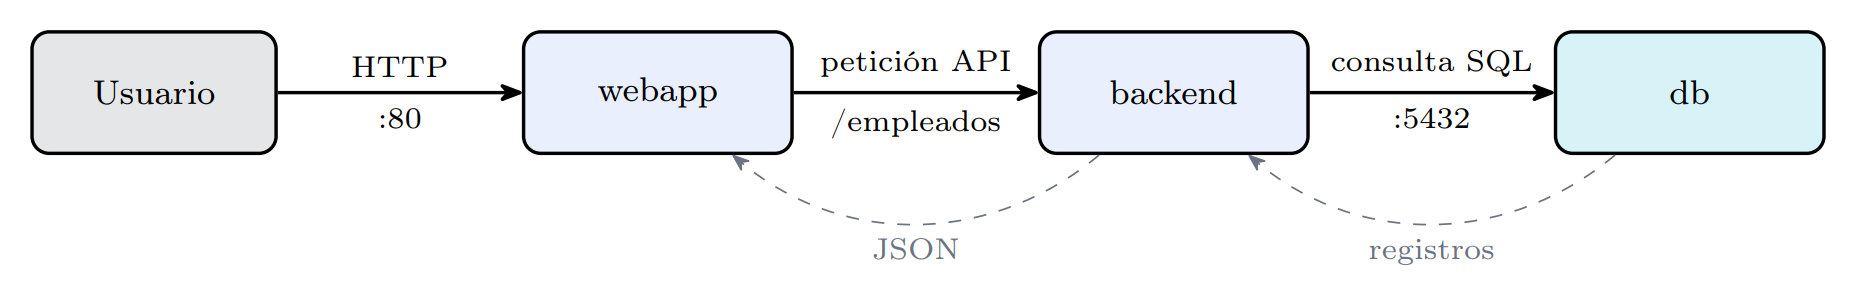
\includegraphics[width=0.9\linewidth]{img/cap04-flujo-microservicios.jpg}
            \caption{Flujo de peticiones entre \texttt{webapp}, \texttt{backend} y \texttt{db}, con puertos de comunicación.}
            \label{fig:flujo-microservicios}
        \end{figure}
        
        \subsection{Tecnología utilizada}
        Docker\footnote{\url{https://www.docker.com}} es el pilar fundamental de la tecnología utilizada en este trabajo. Es el responsable del despliegue y la gestión de los contenedores, así como de la creación de las redes y de las reglas que las conectan \cite{dockernet}. Al tratarse de la tecnología de contenedores más extendida y considerada un estándar de facto en infraestructuras contenerizadas, existe abundante documentación académica y técnica al respecto, y el autor del trabajo cuenta con experiencia previa en su uso, lo que reduce el coste de aprendizaje.

        Nginx\footnote{\url{https://nginx.org}} es un servidor web y proxy inverso ampliamente utilizado. En el trabajo desempeña dos funciones: en ambos escenarios publica el portal de `webapp` y actúa como punto de entrada desde el exterior, en el Escenario B asume además el papel de punto de aplicación de políticas, al terminar las conexiones mutuamente autenticadas y rechazar las que no acreditan una identidad válida.

        Python\footnote{\url{https://www.python.org}} es el lenguaje elegido para los servicios de aplicación. Su sintaxis legible y el amplio acceso a librería de código permiten implementar la lógica mínima imprescindible con poco esfuerzo, lo que acorta el tiempo de desarrollo y mantiene el foco en la comparación de redes. El autor parte de experiencia previa con el lenguaje, lo que disminuye el coste de aprendizaje.

        Flask\footnote{\url{https://flask.palletsprojects.com}} es un microframework web para Python. Frente a alternativas más completas como Django, prescinde de componentes que este trabajo no necesita y mantiene la reducción de complejidad que buscamos. Tanto `webapp` como `backend` exponen sus rutas HTTP mediante Flask.

        PostgreSQL\footnote{\url{https://www.postgresql.org}} es el sistema gestor de bases de datos relacional que almacena los registros de empleados. Lo elegimos por ser un motor maduro, de código abierto y habitual en entornos productivos, lo que aporta realismo al activo que el atacante intenta alcanzar en la fase post-explotación.

        
    \section{Escenario A — Arquitectura Perimetral}
    En esta sección diseñaremos la red "base" sobre la que implementaremos las mejores del \cref{sec:4.3.1}
        
        \subsection{Topología de red}
        \begin{figure}[ht]
            \centering
            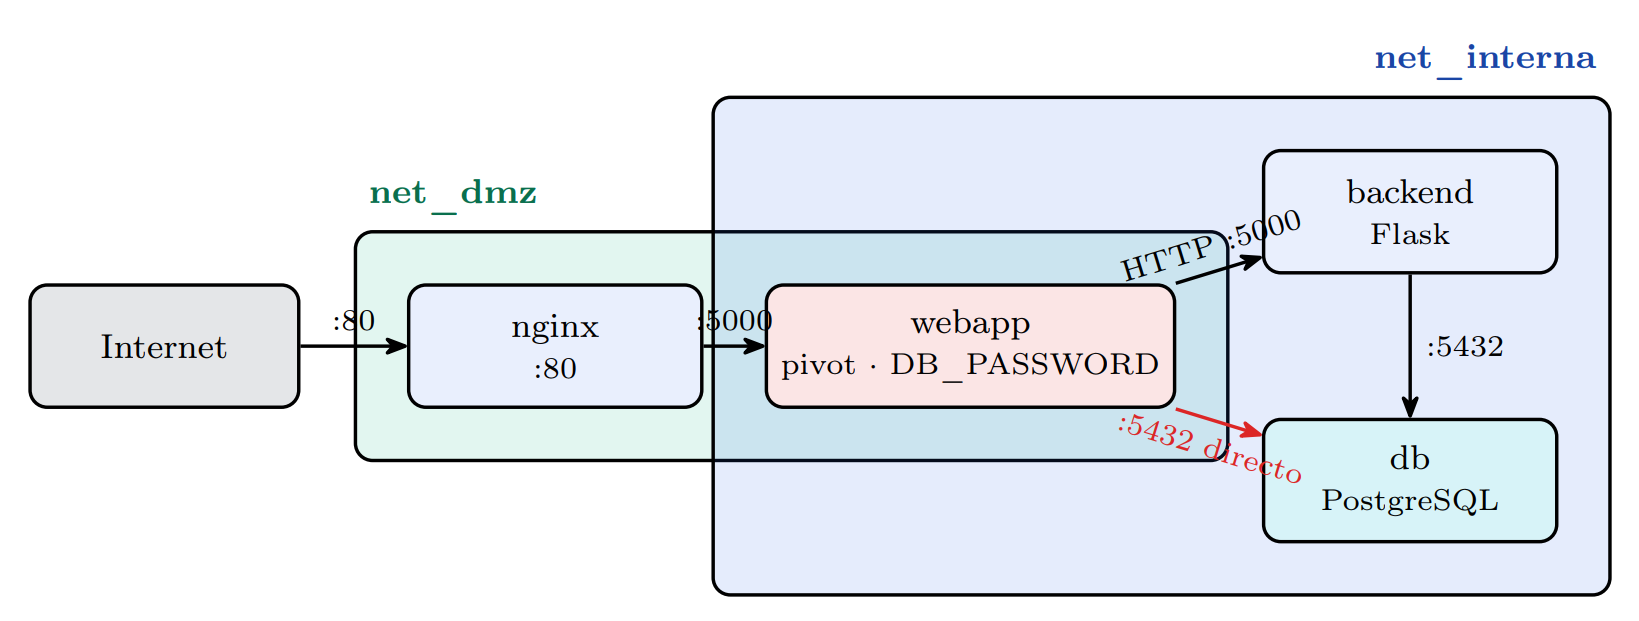
\includegraphics[width=0.9\linewidth]{img/cap04-topologia-perimetral.jpg}
            \caption{Topología del Escenario A: redes \texttt{net\_dmz} y \texttt{net\_interna} con contenedores y flujos permitidos.}
            \label{fig:topologia-perimetral}
        \end{figure}
        
        El Escenario A se organiza en dos redes docker: `net\_dmz` y `net\_interna`. Nginx es el único servicio con puerto expuesto al host (`:80`) y actúa como punto de entrada desde internet.
        
        La aplicación web vulnerable (`webapp`) está en `net\_dmz` y, además, en `net\_interna`: actúa como pivot porque puede comunicarse con ambos segmentos sin control adicional entre ellos. 
        
        En `net\_interna` residen el backend (API Flask) y PostgreSQL con los datos de prueba.
        
        \subsection{Decisiones de diseño}
        Elegimos dos redes (`net\_dmz` y `net\_interna`) porque reproducen una práctica habitual: cortafuegos exterior, servidores web en una zona expuesta y datos en una red interna "protegida".
        
        La segmentación existe, pero se concentra en el perímetro: dentro de la red interna no hay verificación de identidad entre servicios ni monitorización del movimiento lateral.
        
        Este escenario no pretende ser seguro; es la referencia contra la que medimos la mejora. A propósito dejamos `DB\_PASSWORD` en el entorno de `webapp` y el tráfico hacia el backend en HTTP plano por el puerto 5000, de modo que los cuatro hitos post-explotación del protocolo de pruebas sean alcanzables. 
        
        Tampoco desplegamos mecanismos de detección o respuesta, ni sistema de gestión de eventos de seguridad (SIEM), ni cortafuegos de aplicación web (WAF), ni sistema de detección de intrusiones (IDS): la protección se limita al perímetro exterior.
        
        \subsection{Superficie inicial de comparación}
        \label{sec:4.2.3}

        Una vez obtenida la reverse shell en `webapp`, el atacante ejecuta siempre la misma secuencia de cuatro hitos post-explotación, definida en el \cref{sec:3.2.4}: exfiltración de credenciales del entorno del contenedor, escaneo de la red interna, acceso al endpoint `/empleados` del backend y volcado de la tabla de empleados en PostgreSQL.
        
        Esta secuencia es el denominador común entre ambas arquitecturas. En el Escenario A los cuatro hitos son alcanzables por diseño, porque ningún control interno los impide, sirven así de baseline frente al que se mide el Escenario B. La ejecución concreta de cada hito y los valores observados se documentan en el capítulo de pruebas (\cref{sec:6.2}).

    \section{Escenario B — Arquitectura Zero Trust}
        \subsection{Principios aplicados}
        \label{sec:4.3.1}
        El Escenario B parte del principio rector de Zero Trust: "nunca confíes, siempre verifica", y lo concreta en tres principios operativos, cada uno traducido a una medida con la que contrarrestar los hitos definidos en \cref{sec:3.2.4}:
        \begin{itemize}
            \item \textbf{Verificación explícita}. Exigimos que cada flujo este-oeste se autentique antes de permitirse: el canal crítico `webapp $\rightarrow$ backend` usa autenticación mutua con certificados (mTLS), de modo que pertenecer a una red ya no equivale a confianza automática.
            \item \textbf{Mínimo privilegio.} Segmentamos la estructura en tres zonas y solo habilitamos los puertos estrictamente necesarios entre zonas contiguas. Las credenciales de la base de datos residen solo en `backend` y `webapp` no recibe `DB\_PASSWORD` en su entorno, lo que corrige el punto débil del escenario perimetral.
            \item \textbf{Asumir brecha.} Diseñamos como si `webapp` ya estuviera comprometida: la segmentación impide el salto directo a la base de datos, el mTLS rechaza las peticiones sin certificado de cliente y Wazuh observa los comandos que el atacante lanza desde la shell post-RCE, aunque los controles de red ya hayan frustrado parte del ataque.
        \end{itemize}
        Estos tres principios son la respuesta de diseño al \textit{Requisito-F 3} (\cref{sec:3.3.1}): que el Escenario B bloquee o, como mínimo, detecte los cuatro hitos post-RCE alcanzables en el perimetral.
        
        \subsection{Topología de red}
        \begin{figure}[ht]
            \centering
            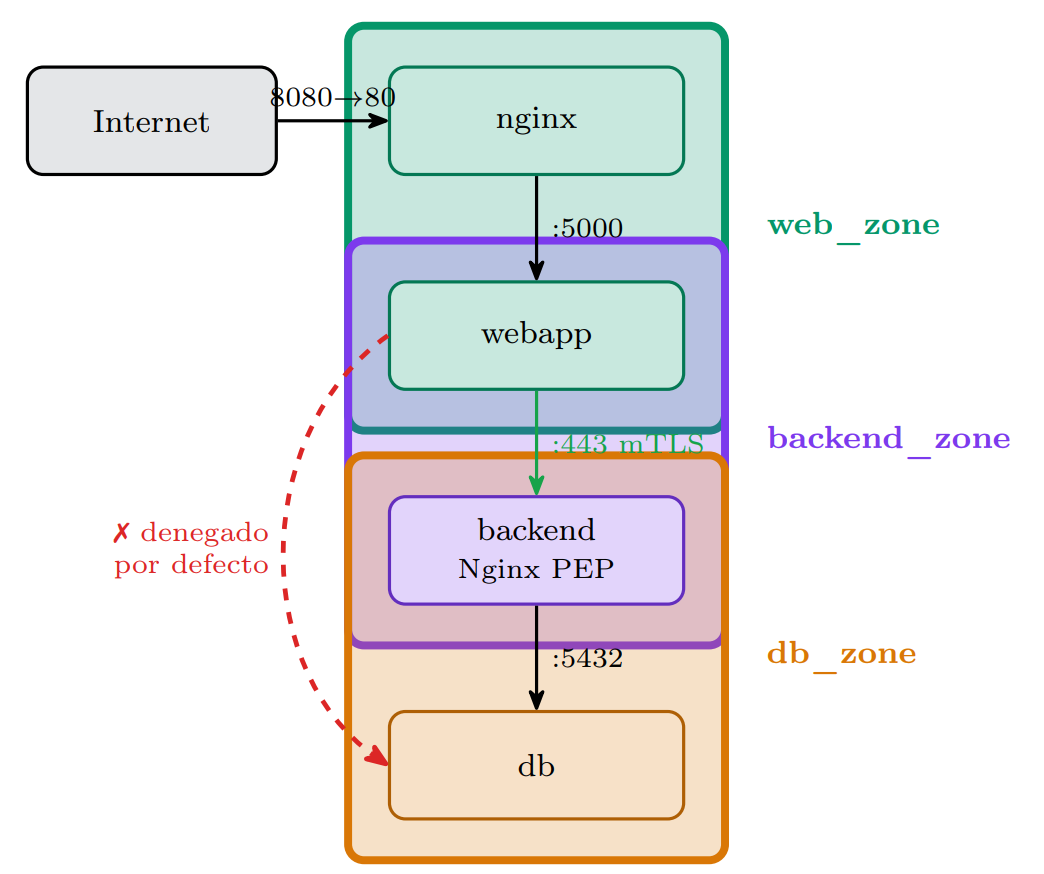
\includegraphics[width=0.9\linewidth]{img/cap04-topologia-zerotrust.jpg}
            \caption{Topología del Escenario B: zonas \texttt{web\_zone}, \texttt{backend\_zone} y \texttt{db\_zone} con microsegmentación.}
            \label{fig:topologia-zerotrust}
        \end{figure}

        Frente a las dos redes del modelo perimetral, la topología Zero Trust reparte los contenedores en tres zonas aisladas, de modo que cada servicio pertenece únicamente a las zonas que necesita para operar:
        \begin{itemize}
            \item \textbf{web\_zone}: agrupa nginx y `webapp`; es la única zona accesible desde el exterior.
            \item \textbf{backend\_zone}: comunica `webapp`, como cliente, con `backend`, como servidor; es el canal sobre el que se aplica mTLS.
            \item \textbf{db\_zone}: comunica `backend` con la base de datos `db`.
        \end{itemize}

        Los flujos permitidos entre zonas son los siguientes:
        \begin{itemize}
            \item entrada externa únicamente a nginx (puertos: 8080 $\rightarrow$ 80)
            \item nginx $\rightarrow$ webapp en el puerto 5000
            \item webapp $\rightarrow$ backend por HTTPS en el 443, con terminación mTLS en Nginx del contenedor backend
            \item backend $\rightarrow$ PostgreSQL en el 5432. 
        \end{itemize}
        
        No existe ruta webapp $\rightarrow$ db porque ningún servicio tiene interfaz en `web\_zone` y `db\_zone` a la vez. 
        
        Cualquier comunicación no enumerada se considera denegada por defecto.

        Además, la conexión entre webapp $\rightarrow$ backend queda encriptada gracias a https y verificada por mTLS.
        
        \subsection{mTLS entre webapp y backend}
        \begin{figure}[ht]
            \centering
            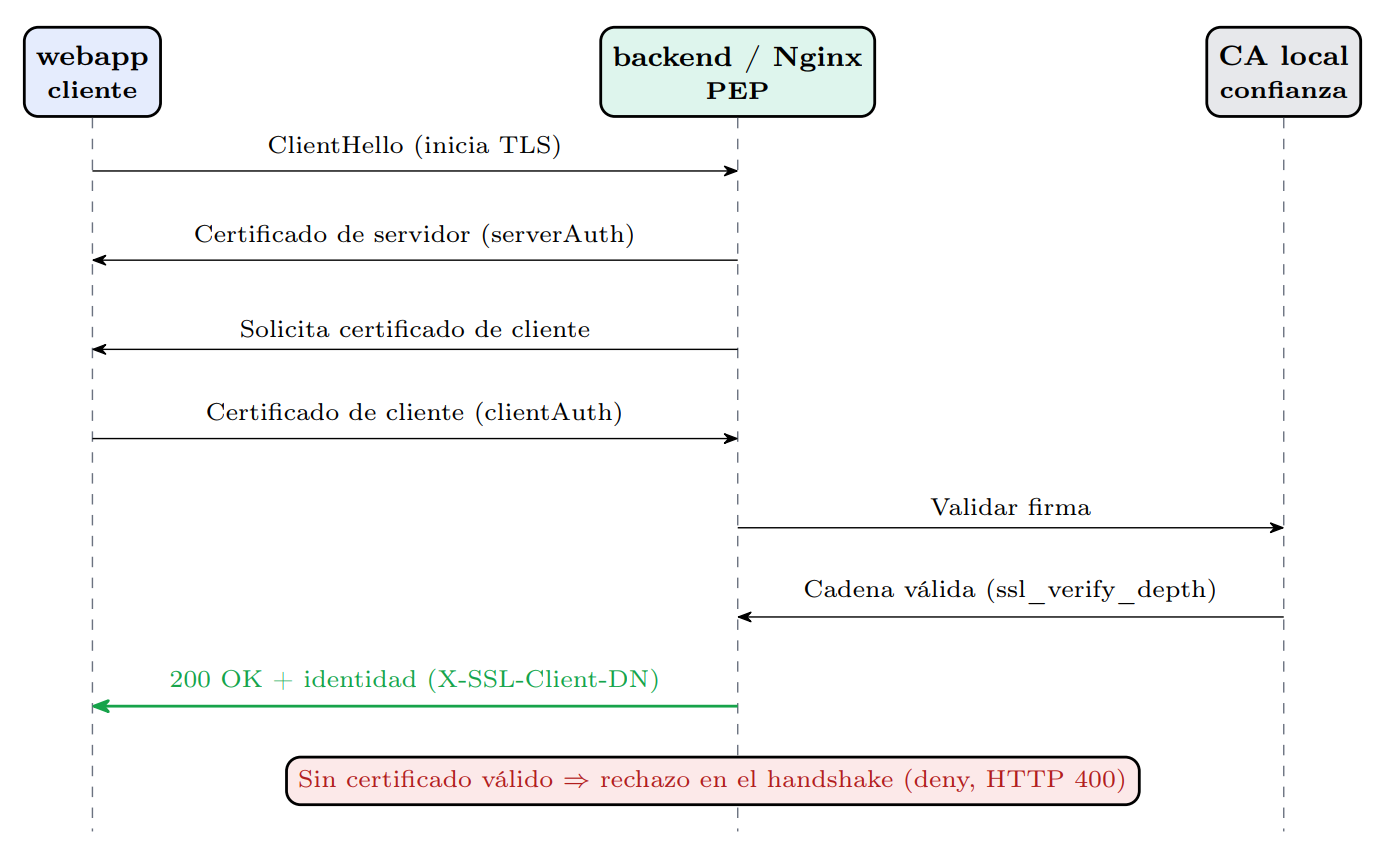
\includegraphics[width=0.9\linewidth]{img/cap04-mtls-handshake.jpg}
            \caption{Secuencia de autenticación mutua (mTLS) entre \texttt{webapp} y \texttt{backend} mediante certificados firmados por una CA local.}
            \label{fig:mtls-handshake}
        \end{figure}
        
        En el Escenario A el tráfico de `webapp` a `backend` viaja en HTTP plano por el puerto 5000. En el Escenario B lo ciframos y autenticamos con mTLS, una variante de TLS en la que no solo el servidor presenta certificado, sino que también el cliente debe acreditar su identidad. Una autoridad de certificación (CA) local, generada con OpenSSL, firma un certificado de servidor para `backend` y un certificado de cliente para `webapp`.
        
        Nginx, desplegado en el contenedor `backend`, actúa como punto de aplicación de políticas (PEP): solo admite la conexión si el cliente presenta un certificado válido firmado por esa CA; en caso contrario, la rechaza. De este modo, el simple hecho de alcanzar la red del backend ya no basta para hablar con la API. Los detalles de configuración de Nginx y del montaje de certificados se documentan en \cref{sec:5.3.3}.
        
        \subsection{Observabilidad activa — Wazuh}
        \label{sec:4.3.4}
        \begin{figure}[ht]
            \centering
            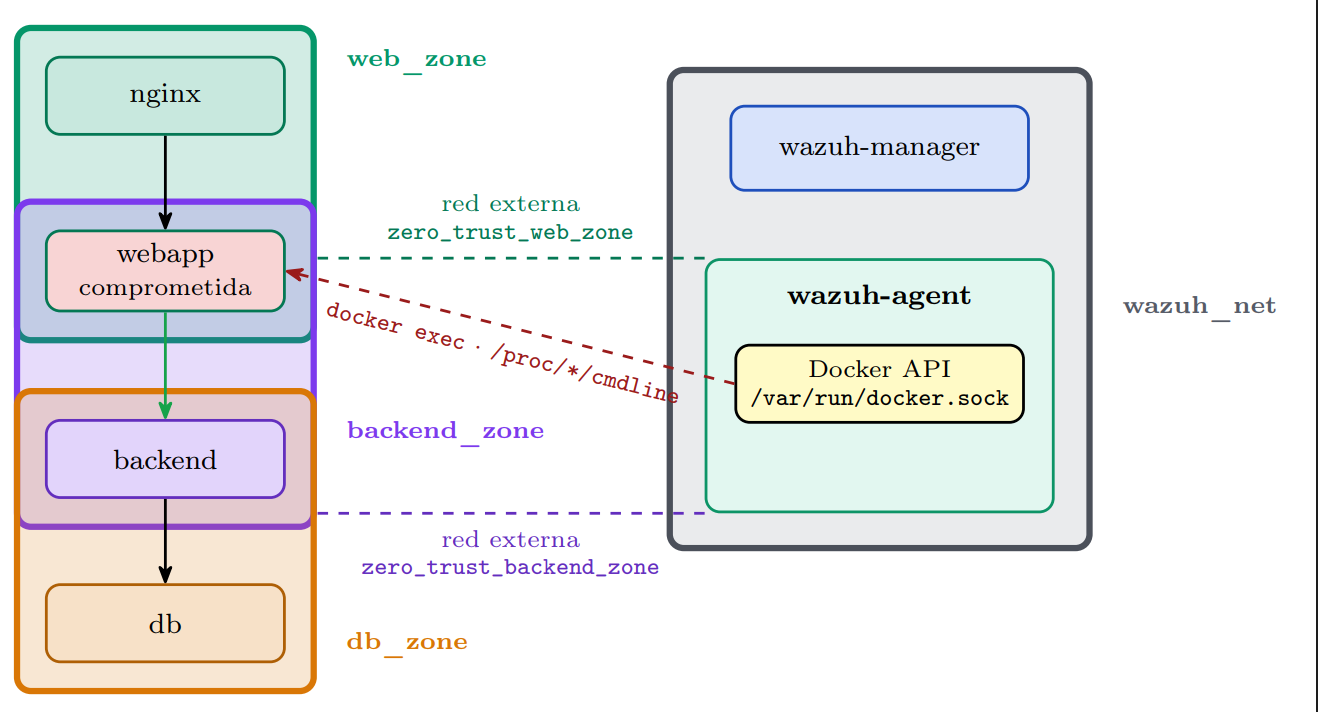
\includegraphics[width=0.9\linewidth]{img/cap04-wazuh-zerotrust.jpg}
            \caption{Integración de Wazuh (manager y agente) en el stack Zero Trust y redes observadas.}
            \label{fig:wazuh-zerotrust}
        \end{figure}
        
        Como objetivo secundario se propuso añadir observabilidad al escenario Zero Trust.
        
        Para la detección activa desplegamos Wazuh en dos contenedores, manager y agente. El agente se sitúa en el socket de Docker y observa los procesos que se ejecutan dentro de webapp.

        Definimos reglas locales alineadas con los cinco patrones de actividad: escaneo nmap, curl hacia backend, tcpdump, psql y grep de patrones de credenciales. La microsegmentación y el mTLS bloquean el impacto. Luego Wazuh registra el intento y permite medir tiempos. 

    \section{Tecnología utilizada en Zero Trust}
    El Escenario B incorpora tres tecnologías que no intervienen en el modelo perimetral:

    mTLS (Mutual TLS) es una extensión del protocolo TLS en la que no solo el servidor presenta un certificado al cliente, sino que el cliente también debe acreditar el suyo. De este modo, ambos extremos verifican su identidad antes de intercambiar datos. En este trabajo, esa exigencia convierte la pertenencia a una red en una condición insuficiente para comunicarse: solo los servicios que presentan un certificado válido pueden hacerlo.

    OpenSSL\footnote{\url{https://www.openssl.org}} es una biblioteca y un conjunto de herramientas de línea de comandos de código abierto para operaciones criptográficas. La empleamos para crear la autoridad de certificación (CA) local y emitir los certificados de servidor y de cliente que sustentan el mTLS, sin depender de una infraestructura de clave pública externa.

    Wazuh\footnote{\url{https://wazuh.com}} es una plataforma de seguridad de código abierto orientada a la detección basada en host (HIDS, \textit{Host-based Intrusion Detection System}). Recoge y analiza la actividad de los sistemas vigilados y genera alertas cuando esa actividad coincide con un conjunto de reglas. En el experimento aporta la capa de observabilidad activa del Escenario B: vigila los procesos que se ejecutan dentro de `webapp` tras la intrusión y registra los comandos del atacante, lo que permite medir el indicador de detección.

        \subsubsection{Decisión de tecnología}
        La iteración inicial del trabajo contemplaba Suricata\footnote{\url{https://suricata.io}} como sonda de red. Lo descartamos porque nuestro modelo de amenazas fija la ejecución de código remota en webapp y los hitos comparativos ocurren como comandos dentro del contenedor (nmap, curl, psql, grep), no solo como patrones de tráfico observables en la red.

        Wazuh aporta detección host-based sobre esos procesos mientras que Suricata es network-based y no sustituye la visibilidad del cmdline en el namespace del contenedor comprometido. Para este alcance del TFG la elección es más relevante que combinar ambas capas. 
        
        Dejamos Suricata como línea futura de detección a nivel de red, actuaría junto a Wazuh, complementándolo y no sustituyéndolo.
    
    \FloatBarrier
    \section{Limitaciones del diseño}
    \label{sec:4.5}


    Reconocemos varias limitaciones de este diseño en el entorno de laboratorio, entre ellas:

    \begin{enumerate}
        \item El mTLS solo cubre el canal webapp $\rightarrow$ backend mientras que los flujos nginx $\rightarrow$ webapp y backend $\rightarrow$ db siguen sin cifrado mutuo.
        \item Los certificados son autofirmados. Además, mTLS verifica la identidad del servicio, pero no define qué operaciones puede ejecutar cada certificado una vez autenticado.
        \item Wazuh se despliega sin Indexer ni dashboard: las alertas se vuelcan a un json manualmente y no disparan respuesta automática (no hay SOAR) y el agente usa muestreo cada 2 s mediante `process-webapp`, no trazado syscall en tiempo real.
        \item El entorno de trabajo es Docker local en Windows/WSL2, no un clúster Kubernetes productivo: los resultados son representativos del contraste perimetral vs Zero Trust en contenedores, pero no se extrapolan directamente a despliegues cloud-native a escala.
    \end{enumerate}

\FloatBarrier
%%%%%%%%%%%%%%%%%%%%%%%%%%%%%%%%%%%%%%%%%%%%%%%%%%%%%%%%%%%%%


\chapter{Desarrollo e implantación de la solución}
    
    \section{Infraestructura como código}
    El capítulo de diseño fijó la topología, los controles y la tecnología empleada. En este capítulo describimos cómo trasladamos ese diseño a contenedores Docker ejecutables: cómo desarrollamos los servicios, cuáles desplegamos y qué decisiones tomamos cuando la implementación encontró restricciones del entorno de laboratorio.
    
    Hemos representado los dos escenarios comparativos como dos conjuntos de Docker Compose independientes. Cada servicio, red y variable de entorno queda definido en ficheros de configuración versionados, de modo que cualquier sesión puede reproducirse desde un estado conocido con el comando:
    
    \begin{lstlisting}[language=Bash, aboveskip=10pt, belowskip=10pt]
docker compose up --build
    \end{lstlisting}
    
    \section{Red Perimetral}
    
        \subsection{Desarrollo de la aplicación}
        Como ya hemos mencionado en el diseño (\cref{sec:4.1.1}) el desarrollo de la app web es relativamente sencillo.
        \begin{itemize}
            \item \textbf{Nginx:} se configura con un simple archivo \texttt{nginx.conf} que establece que el servidor web escucha en el puerto :80 (\cref{fig:nginxconf}).

           \begin{figure}[H]
                \centering
                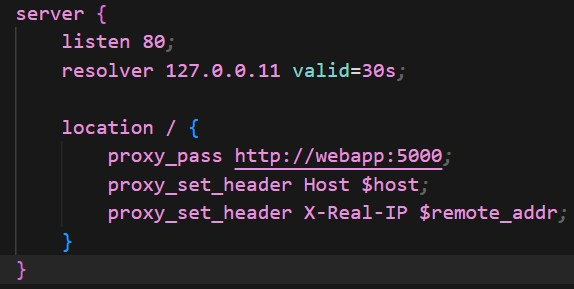
\includegraphics[width=0.7\linewidth]{img/nginxconf.jpg}
                \caption{\texttt{nginx.conf} del punto de entrada: proxy inverso hacia \texttt{webapp}.}
                \label{fig:nginxconf}
            \end{figure}
            
            \item Para \textbf{webapp} y \textbf{backend}: ambos son implementados por un script Python que importa e implementa Flask. El código de \texttt{app.py} en cada servicio figura en el anexo \cref{anexo:codigo_aplicacion}.
            \item La \textbf{base de datos} se inicializa con un \texttt{init.sql}, también incluido en \cref{anexo:codigo_aplicacion}.
        \end{itemize}
        
 
        
        \subsection{Implementación de la app web en la red perimetral}
        Para que Docker pueda desplegar cada microservicio en la red como contenedores, se deben crear ``imágenes'' de ejecución (véase el \ref{anexo:docker}).

        Para agilizar el proceso de desarrollo, docker permite descargar imágenes predefinidas, aprovechando esto y dado el hecho de que nginx y la base de datos solo requieren de configuración y no de desarrollo, utilizamos esta funcionalidad.

        Por otro lado, como webapp y backend son aplicaciones propias, requerimos crear las imágenes nosotros. Esto lo logramos mediante unos archivos 'Dockerfile' (véase el \ref{anexo:docker}), los cuales se encargan de construir la imagen a la que pasan el código fuente python para su ejecución.

        % \begin{figure}[ht]
        %     \centering
        %     \includegraphics[width=0.85\linewidth]{img/cap05-dockerfile.jpg}
        %     \caption{\texttt{Dockerfile} de \texttt{webapp} o \texttt{backend} para construir la imagen de ejecución.}
        %     \label{fig:dockerfile}
        % \end{figure}
        
        \subsection{Punto de entrada: cadena hasta la ejecución remota}
        \label{sec:5.2.3}
        El diseño exige un atacante externo que, tras comprometer \texttt{webapp}, inicie la ventana de medición post-explotación. En la implementación materializamos ese acceso inicial con una cadena de varios eslabones que reproduce debilidades habituales recogidas en el OWASP Top 10 \cite{owasptop10} y termina en ejecución remota mediante una inyección de plantillas del lado del servidor (SSTI) en Jinja2 \cite{owaspssti,cwe1336}.

        Cada eslabón se apoya en una debilidad que introdujimos de forma deliberada en la aplicación. Para nombrarlas con precisión las clasificamos según el catálogo \textit{Common Weakness Enumeration} (CWE), que asigna un identificador a cada \emph{tipo} de debilidad de software, el identificador no describe el ataque, sino la clase de fallo que lo hace posible. Conviene subrayar que todas estas debilidades pertenecen a la fase de acceso inicial: sirven para situar al atacante ante una \textit{reverse shell} en \texttt{webapp}, pero quedan fuera de la ventana de medición comparativa (\cref{sec:6.1.3}). La cadena, paso a paso, es la siguiente:
        \begin{enumerate}
            \item \textbf{Reconocimiento HTTP del portal.} El atacante enumera rutas y respuestas del servidor en busca de puntos de entrada poco protegidos (\cref{fig:pre-rce-escaneo}).

            \begin{figure}[H]
                \centering
                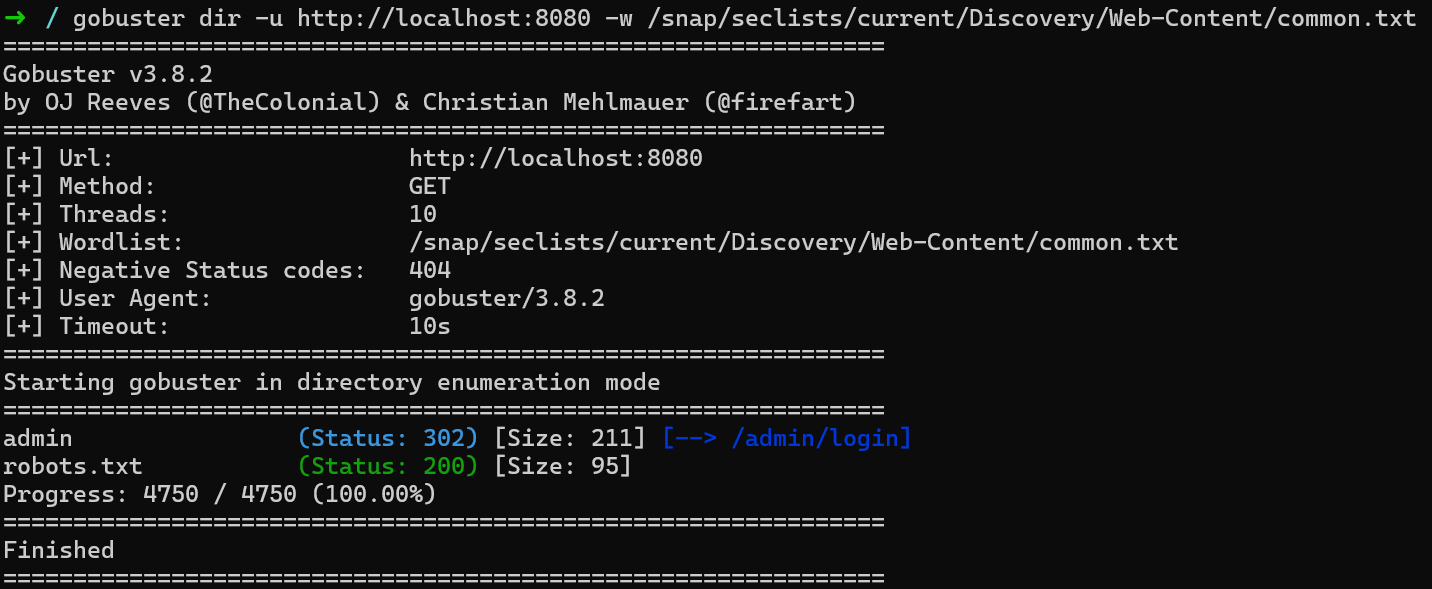
\includegraphics[width=0.85\linewidth]{img/cap05-pre-rce-escaneo.jpg}
                \caption{Reconocimiento HTTP y descubrimiento de rutas antes del RCE.}
                \label{fig:pre-rce-escaneo}
            \end{figure}
            
            \item \textbf{Descubrimiento de rutas internas en \texttt{robots.txt}.} Este fichero, pensado para indicar a los buscadores qué rutas no deben rastrear, enumera precisamente las rutas sensibles del portal (\texttt{/admin/}, \texttt{/backup.txt}). Como es de acceso público y su cumplimiento depende de la buena voluntad del rastreador —hay crawlers que lo ignoran por completo—, en la práctica funciona como un índice de rutas internas para un atacante. Es un caso de exposición de información sensible a un actor no autorizado (CWE-200) (\cref{fig:pre-rce-robots}).

            \begin{figure}[H]
                \centering
                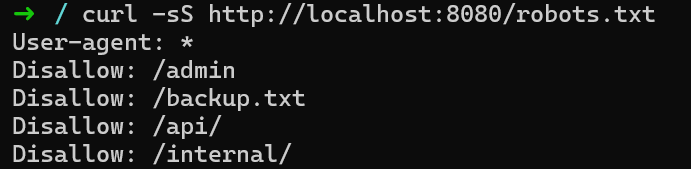
\includegraphics[width=0.85\linewidth]{img/cap05-pre-rce-robots.jpg}
                \caption{Petición \texttt{curl} a \texttt{robots.txt}.}
                \label{fig:pre-rce-robots}
            \end{figure}
            
            \item \textbf{Recuperación de credenciales en \texttt{backup.txt}.} Una de las rutas descubiertas alberga un fichero de respaldo con credenciales de administrador almacenadas en texto claro y accesible desde el exterior: una protección insuficiente de credenciales (CWE-522) (\cref{fig:pre-rce-backup}).

            \begin{figure}[H]
                \centering
                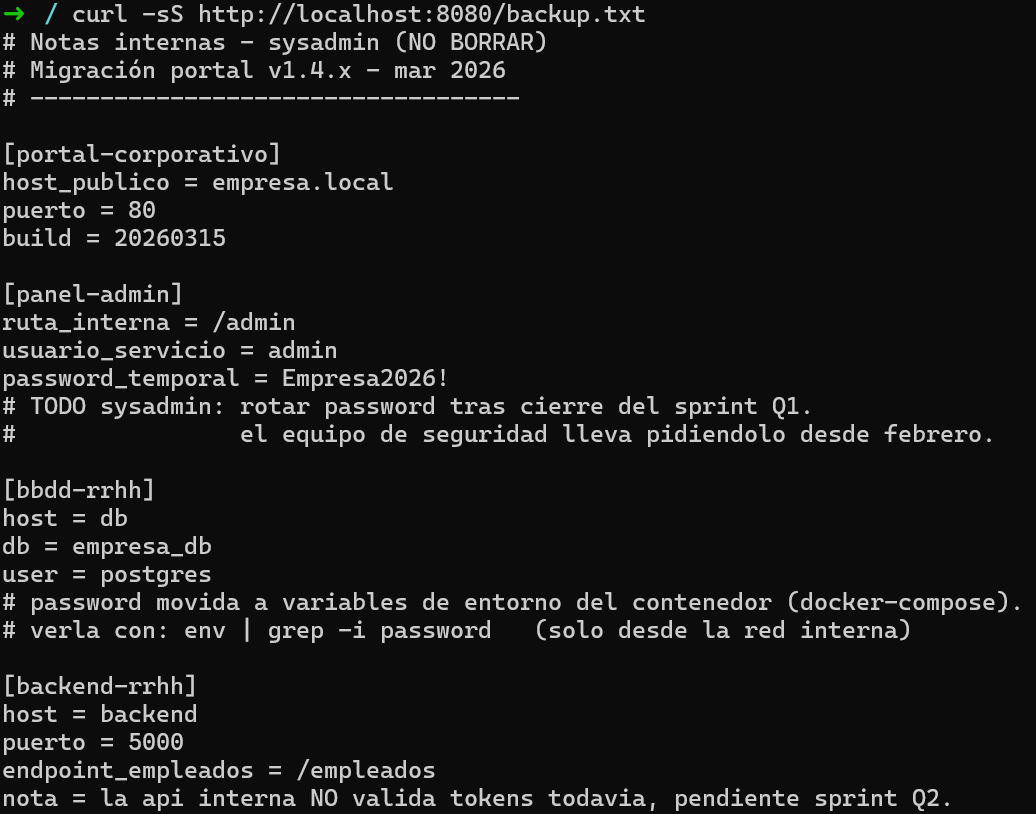
\includegraphics[width=0.85\linewidth]{img/cap05-pre-rce-backup.jpg}
                \caption{Petición \texttt{curl} a \texttt{backup.txt}.}
                \label{fig:pre-rce-backup}
            \end{figure}
            
            \item \textbf{Acceso al panel de administración.} Con esas credenciales el atacante entra en el panel. El acceso se sostiene sobre un único factor, usuario y contraseña, sin un segundo factor que lo respalde una vez filtrada la contraseña (CWE-308) (\cref{fig:pre-rce-dashboard}).

            \begin{figure}[H]
                \centering
                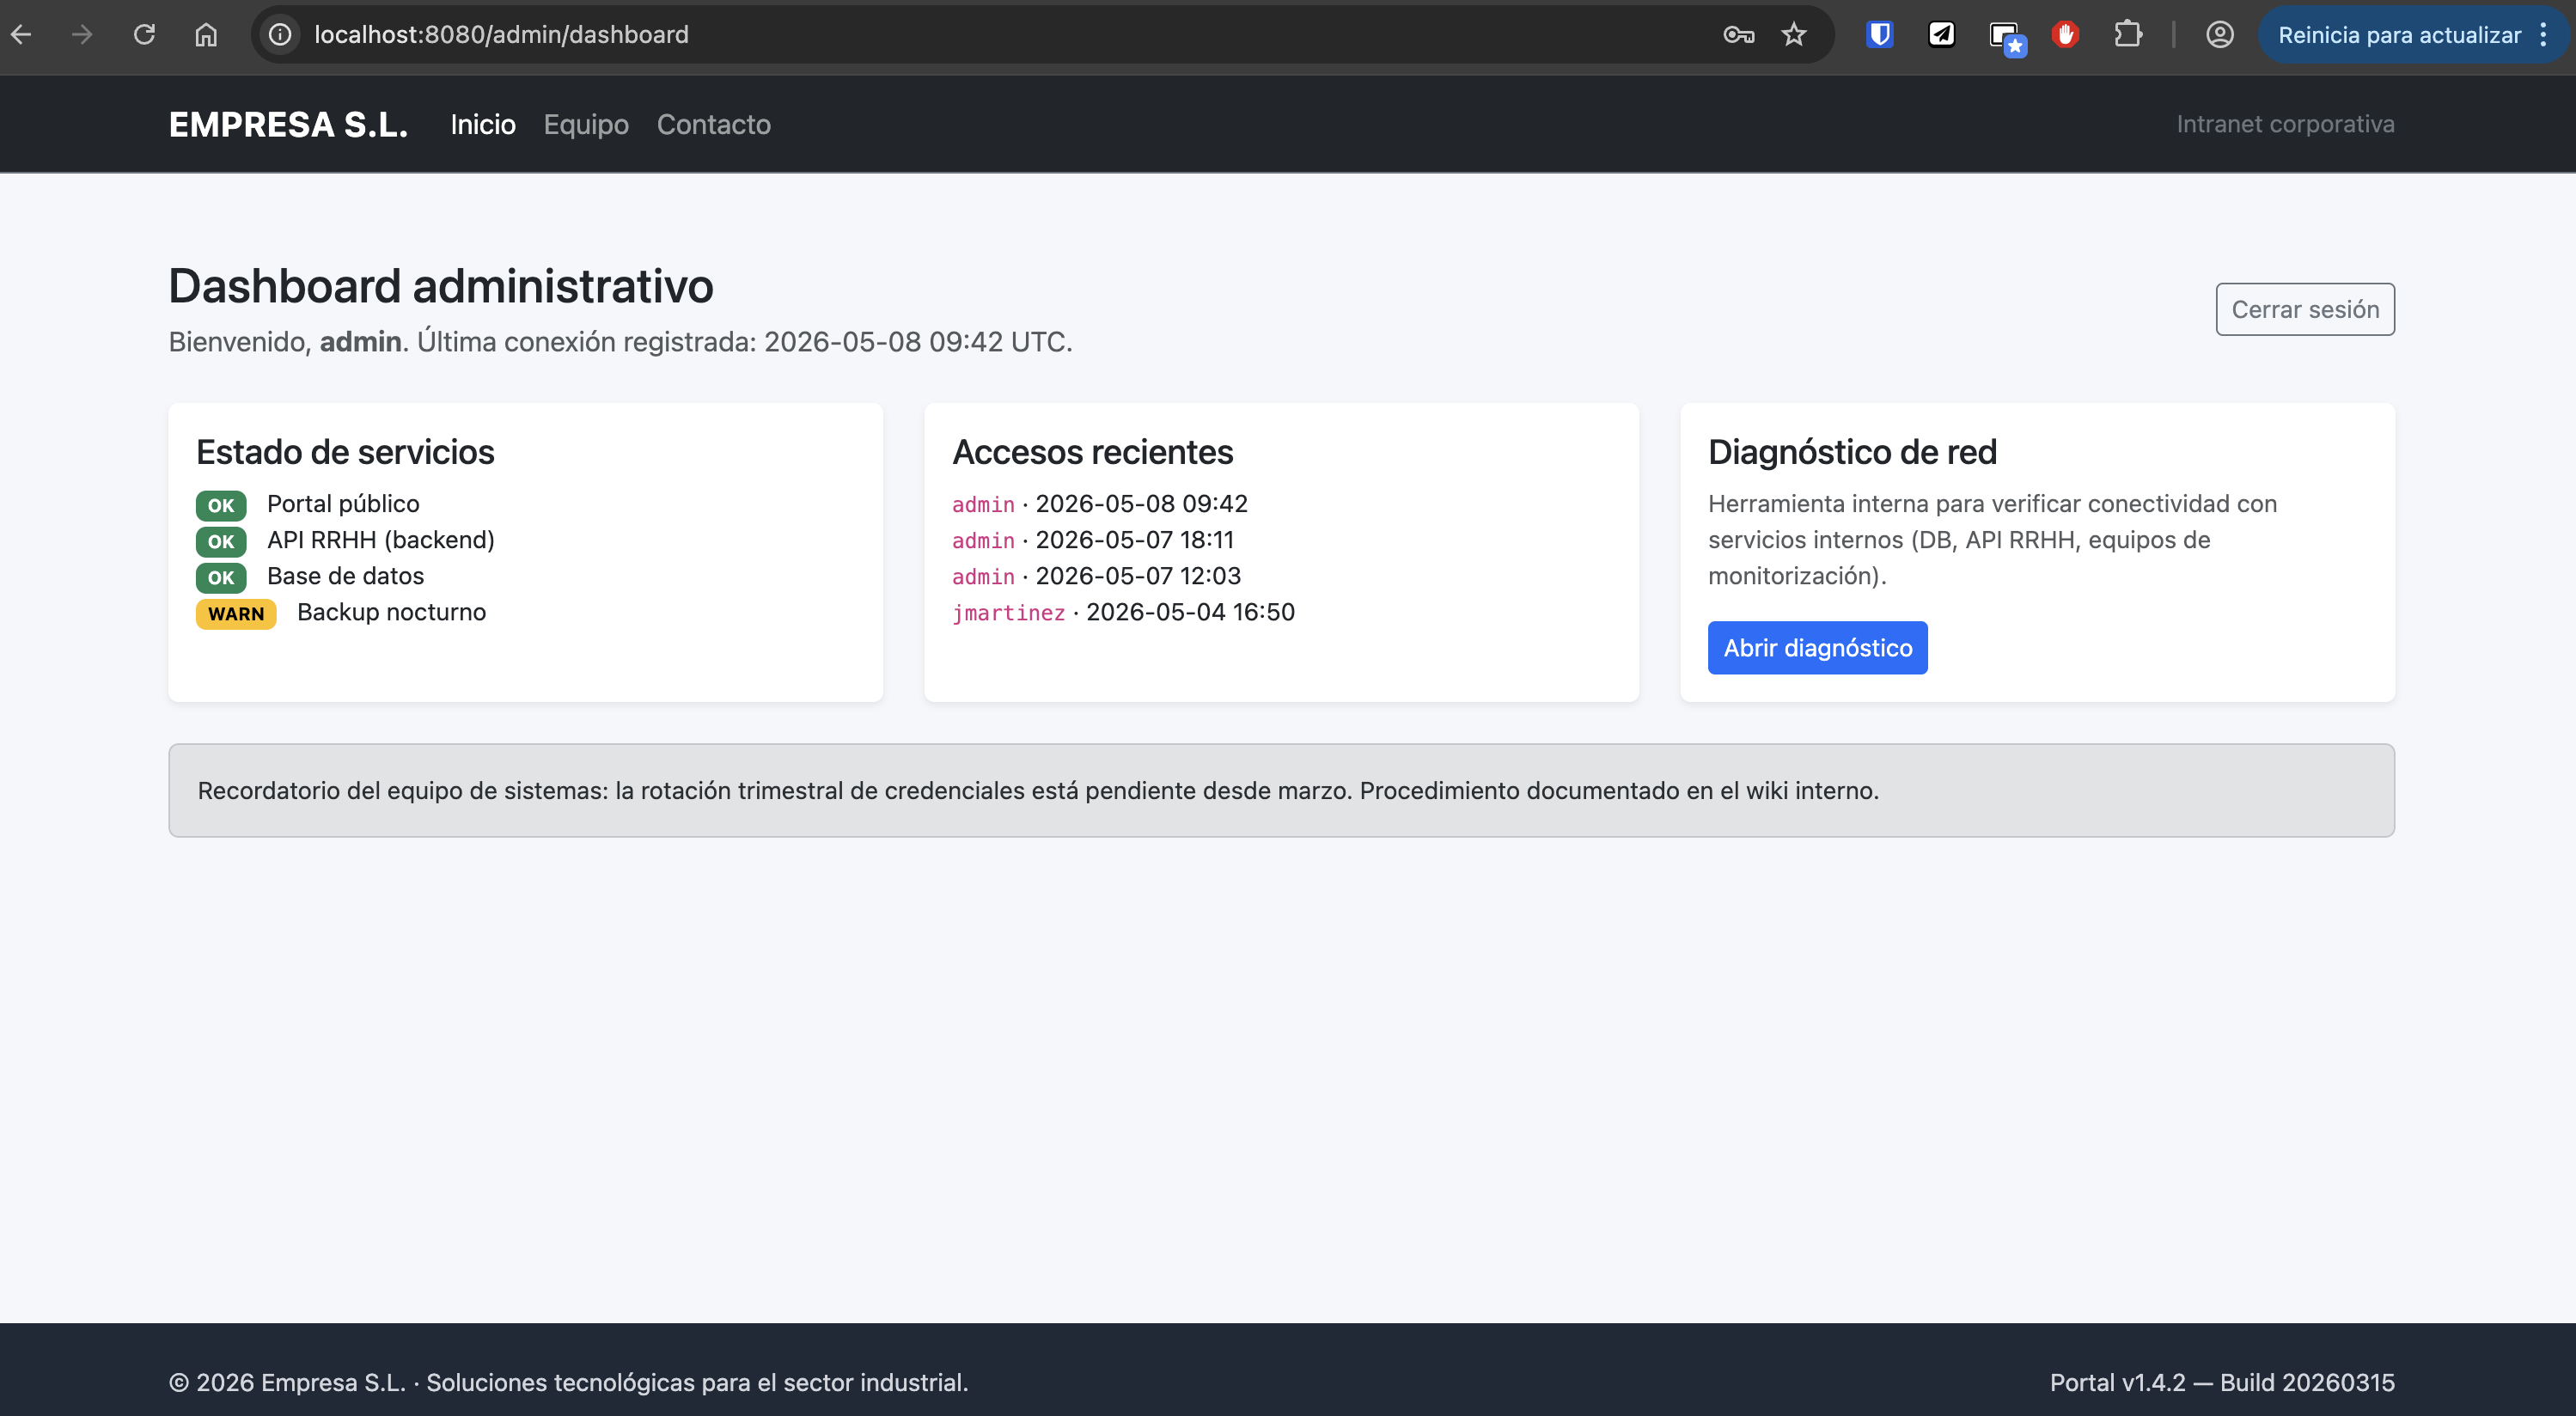
\includegraphics[width=0.85\linewidth]{img/cap05-pre-rce-dashboard.jpg}
                \caption{Panel de administración tras autenticación.}
                \label{fig:pre-rce-dashboard}
            \end{figure}
            
            \item \textbf{Inyección de plantillas y ejecución remota.} En el panel, el parámetro \texttt{host} del endpoint \texttt{/admin/diagnostico} se evalúa como plantilla Jinja2 sin neutralizar la entrada del usuario. Esto habilita una inyección de plantillas del lado del servidor (SSTI, CWE-1336) y, a través de ella, la ejecución remota de código (\cref{fig:pre-rce-ssti}).

            \begin{figure}[H]
                \centering
                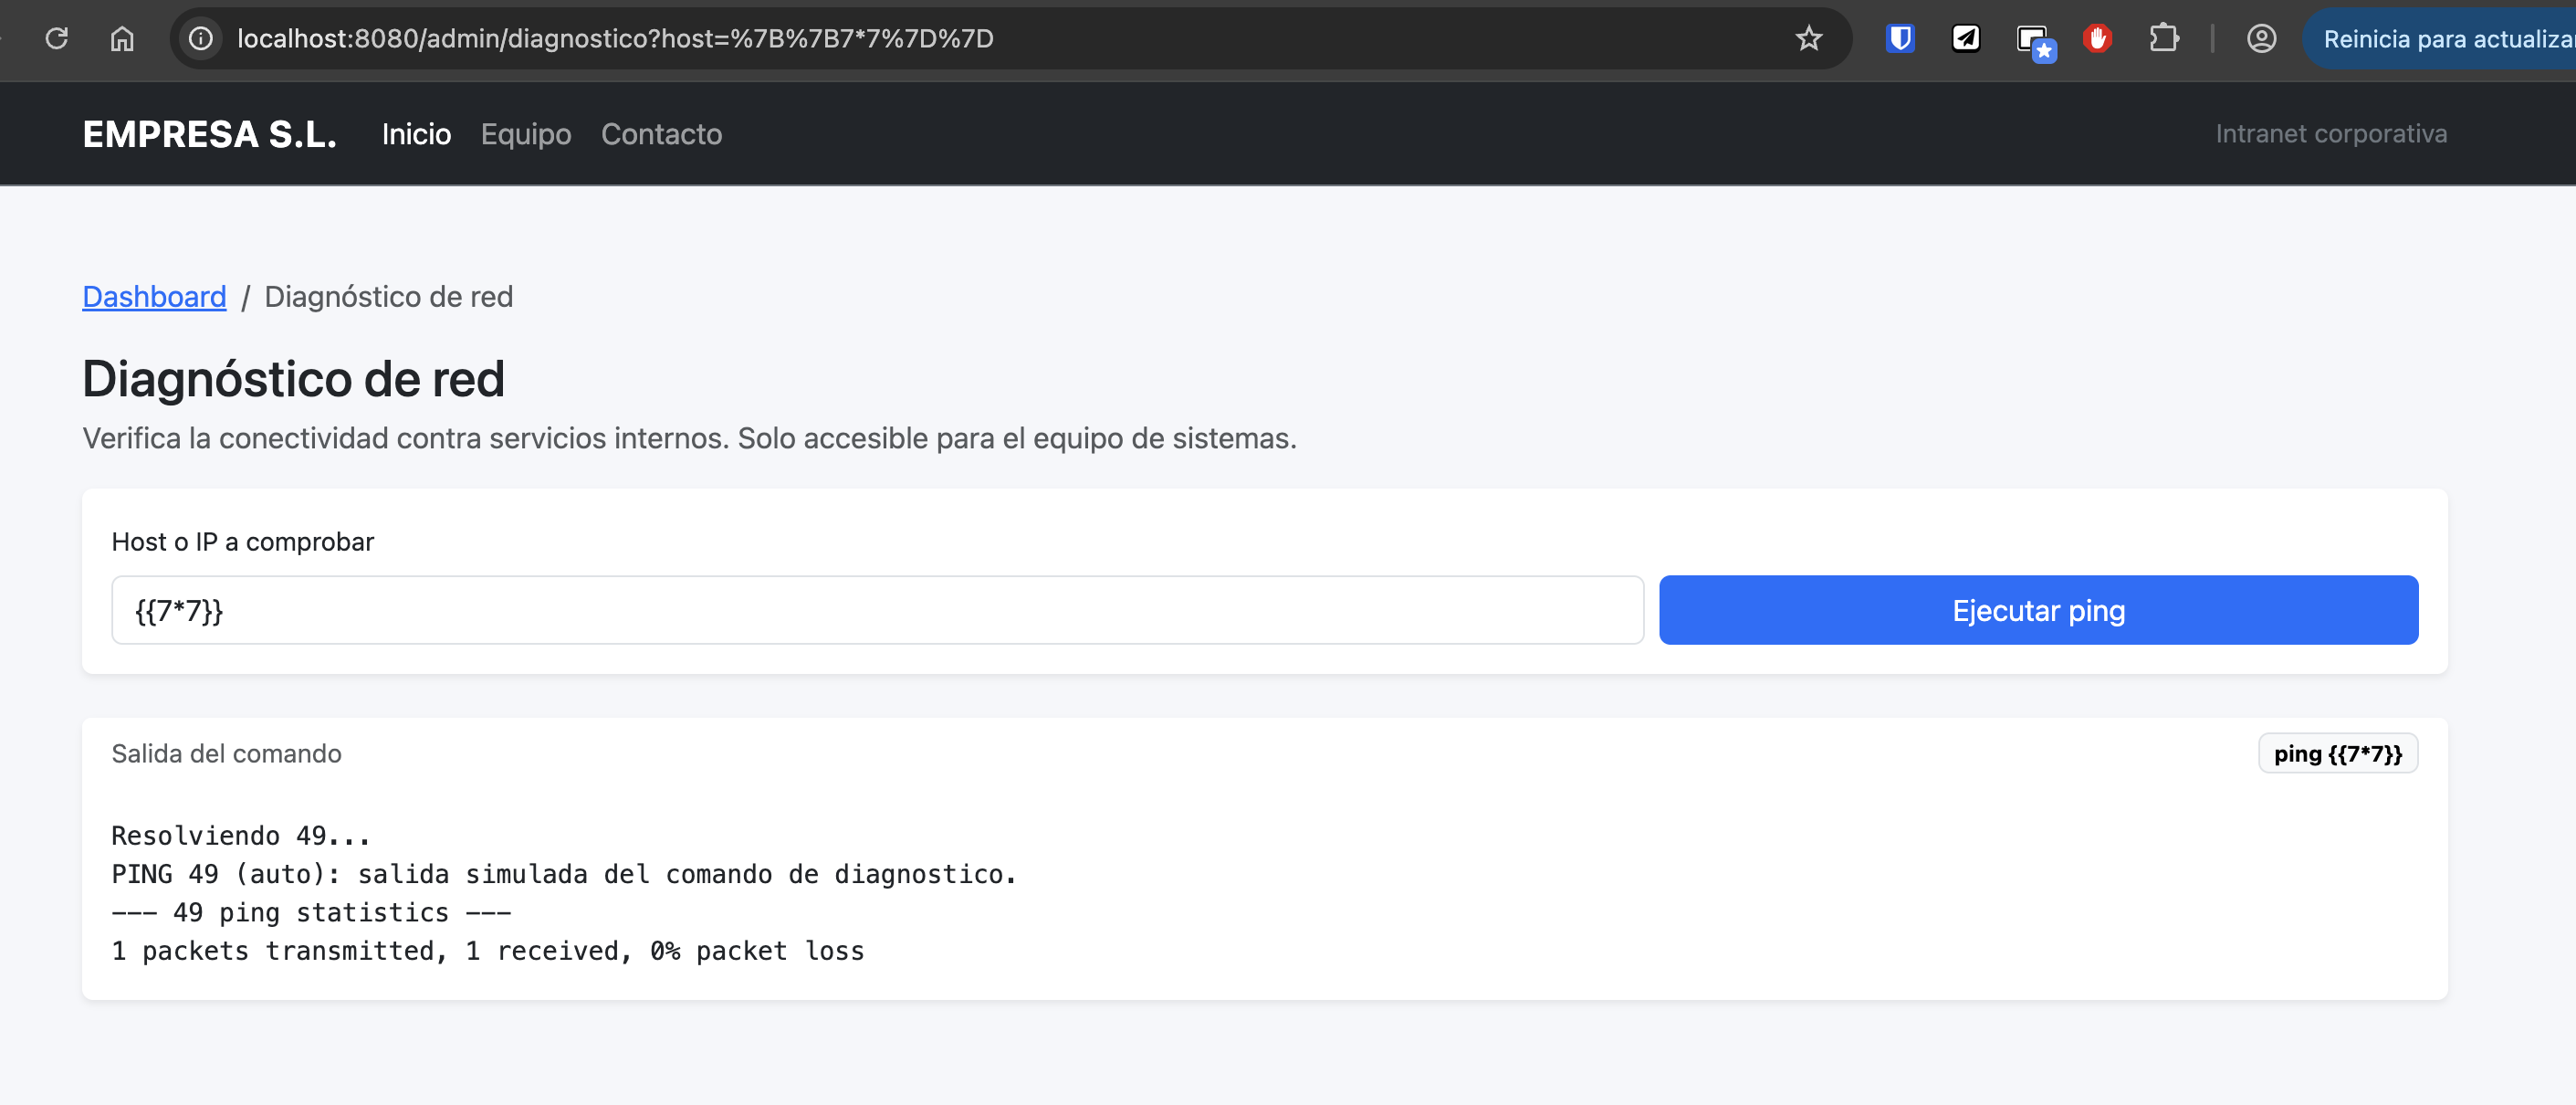
\includegraphics[width=0.85\linewidth]{img/cap05-pre-rce-ssti.jpg}
                \caption{SSTI en Jinja2 y obtención de ejecución remota de comandos.}
                \label{fig:pre-rce-ssti}
            \end{figure}
        \end{enumerate}

        \FloatBarrier
        
        Esta cadena nos permite fijar de forma reproducible el instante en que el atacante dispone de una \textit{reverse shell} en \texttt{webapp}, que es el punto de partida común a ambos escenarios. El detalle de la cadena de ataque y sus resultados corresponde al capítulo de pruebas. Aquí documentamos únicamente que la aplicación se implementó con esos endpoints deliberadamente débiles para habilitar el acceso inicial acordado en el diseño. Importa señalar que ninguna de estas debilidades se corrige en el Escenario B: el punto de entrada es idéntico en ambos, de modo que lo que comparamos no es la facilidad de entrar, sino el alcance del daño una vez dentro.
        
        
        \subsection{Docker Compose}
        Una vez tenemos todo listo para ser contenerizado, utilizamos la herramienta Docker que nos permite gestionar la creación de varios contenedores a la vez: Docker Compose.

        En este archivo de configuración es donde dictamos, para cada contenedor que queremos construir, dónde está la ruta de su imagen (\cref{fig:compose-nginx}) o bien dónde está la ruta con lo necesario para construir dicha imagen (\cref{fig:compose-webapp}).

        \begin{figure}[H]
            \centering
            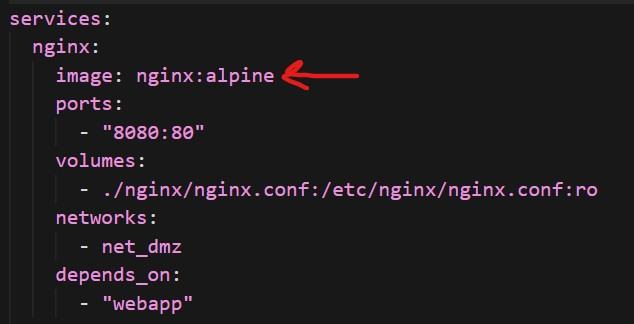
\includegraphics[width=0.6\linewidth]{img/cap05-compose-nginx.jpg}
            \caption{Fragmento del \texttt{docker-compose} — servicio \texttt{nginx}.}
            \label{fig:compose-nginx}
        \end{figure}

        \begin{figure}[H]
            \centering
            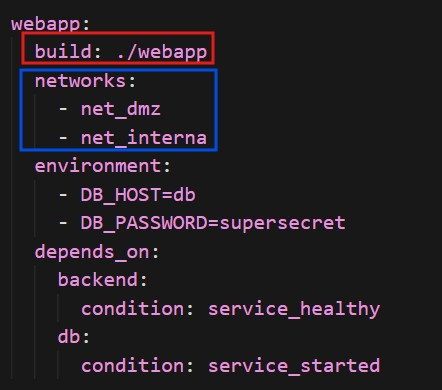
\includegraphics[width=0.5\linewidth]{img/cap05-compose-webapp.jpg}
            \caption{Fragmento del \texttt{docker-compose} — servicio \texttt{webapp} con \texttt{build} y redes asociadas.}
            \label{fig:compose-webapp}
        \end{figure}

        \subsubsection{Redes Docker}
            Lo más relevante para este trabajo en el archivo compose es la creación de las redes Docker internas y la asociación de cada contenedor a su respectiva red, que es lo que materializa la topología diseñada en el capítulo 4 y determina qué contenedores pueden comunicarse entre sí. En \cref{fig:compose-redes} y \cref{fig:compose-webapp} puede observarse cómo cada servicio declara, bajo la clave \texttt{networks}, las redes a las que pertenece: \texttt{webapp} figura a la vez en \texttt{net\_dmz} y en \texttt{net\_interna}, lo que la convierte en el único pivote entre el segmento expuesto y el interno, mientras que \texttt{db} queda confinada a \texttt{net\_interna}.

            \begin{figure}[ht]
                \centering
                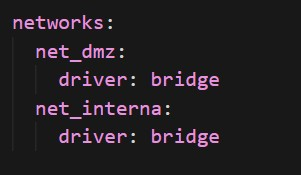
\includegraphics[width=0.4\linewidth]{img/cap05-compose-redes.jpg}
                \caption{Definición de redes en el \texttt{docker-compose} perimetral.}
                \label{fig:compose-redes}
            \end{figure}
        
        \FloatBarrier
        \subsection{Decisiones de implementación}
        \label{sec:5.2.5}

        Durante la implantación del Escenario A tomamos dos decisiones que no figuraban en el diseño inicial, pero que resultaron necesarias para que el laboratorio fuera reproducible:
        \begin{enumerate}
            \item \textbf{Refactor del servicio web con SSTI en Jinja2.} La primera versión implementada exponía un único endpoint con ejecución de comandos. Lo sustituimos por la cadena de acceso inicial documentada en \cref{sec:5.2.3}, que fija un punto de entrada reproducible sin modificar el stack Flask ni añadir contenedores nuevos.
            \item \textbf{Script de captura automatizado.} Los primeros ensayos copiaban los artefactos de forma manual y se perdían al detener el entorno. Automatizamos el proceso con un script (explicado en \cref{sec:5.4.1} y detallado en el anexo \cref{anexo:scripts_captura})
        \end{enumerate}

    \FloatBarrier
    \section{Red Zero Trust}
    Para la red Zero Trust ya tenemos la aplicación web desarrollada, funcionalmente es idéntica y solo requiere unas pequeñas modificaciones que detallaremos a continuación, el mayor cambio se produce a nivel de red.

        \subsection{Segmentación de redes}
        El primer cambio se aplica en el \texttt{docker-compose}, donde sustituimos las dos redes del Escenario A por tres zonas aisladas:
        \begin{enumerate}
            \item \textbf{`web\_zone`} $\rightarrow$ Nginx y `webapp`.
            \item \textbf{`backend\_zone`} $\rightarrow$ `webapp` y `backend`.
            \item \textbf{`db\_zone`} $\rightarrow$ `backend` y `db`.
        \end{enumerate}

        Esto lo conseguimos sustituyendo las redes en el apartado ``networks'' (\cref{fig:zt-compose-networks}).

        \begin{figure}[H]
            \centering
            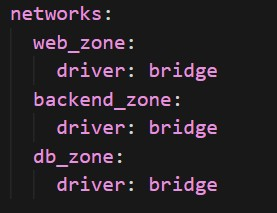
\includegraphics[width=0.4\linewidth]{img/cap05-zt-compose-networks.jpg}
            \caption{Sección \texttt{networks} del \texttt{docker-compose} Zero Trust.}
            \label{fig:zt-compose-networks}
        \end{figure}
        
        De esta forma, `webapp` queda multihomed en `web\_zone` y `backend\_zone`, pero sin interfaz en `db\_zone`, porque la aplicación web no necesita hablar con PostgreSQL: toda la lógica de datos pasa por la API interna de manera exclusiva.
        
        Para comprobar que la segmentación surte efecto lanzamos una prueba de conexión desde \texttt{webapp} a la base de datos, recogida en \cref{fig:zt-segmentacion-test}. A diferencia de una petición hacia \texttt{backend} que se resolvería con normalidad, al compartir ambos \texttt{backend\_zone}, el intento de conexión directa a \texttt{db} agota el tiempo de espera. La diferencia es la clave del control: como \texttt{webapp} no tiene interfaz en \texttt{db\_zone}, la base de datos no es alcanzable ni siquiera por su dirección IP, de modo que la microsegmentación elimina la ruta a nivel de red y no solo la resolución de nombres.

        \begin{figure}[ht]
            \centering
            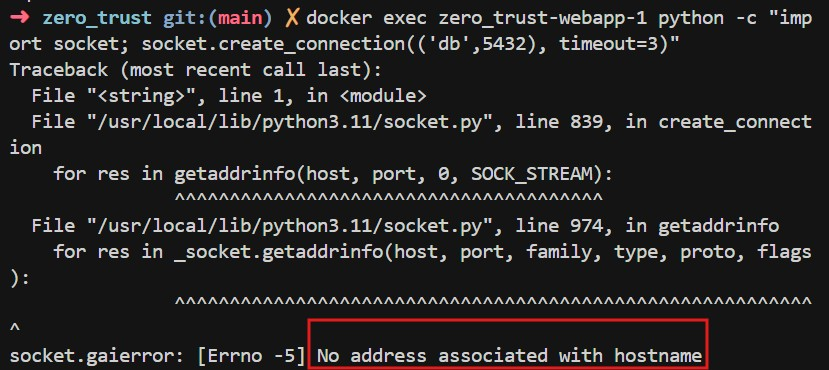
\includegraphics[width=0.7\linewidth]{img/cap05-zt-segmentacion-test.jpg}
            \caption{Verificación de segmentación: \texttt{Intento de conexión a \texttt{db} desde \texttt{webapp}.}}
            \label{fig:zt-segmentacion-test}
        \end{figure}
        
        \subsection{Identidad de servicio y credenciales}
        El diseño exige que comprometer \texttt{webapp} no exponga las credenciales de la base de datos. Para ello modificamos su entorno en el \texttt{docker-compose}: eliminamos \texttt{DB\_HOST} y \texttt{DB\_PASSWORD} y dejamos únicamente la URL del backend cifrado, como muestra \cref{fig:zt-webapp-env}.

        \begin{figure}[H]
            \centering
            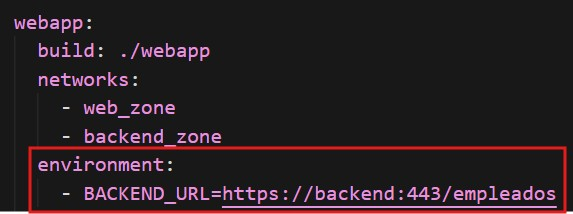
\includegraphics[width=0.7\linewidth]{img/cap05-zt-webapp-env.jpg}
            \caption{Variables de entorno de \texttt{webapp}: \texttt{BACKEND\_URL} sin credenciales de base de datos.}
            \label{fig:zt-webapp-env}
        \end{figure}
        
        Las credenciales de PostgreSQL permanecen solo en `backend`, el único servicio con ruta hacia `db`. 
        
        \subsection{Implementación de mTLS}
        \label{sec:5.3.3}
        El diseño protege el canal `webapp $\rightarrow$ backend` con mTLS. La implantación siguió estos pasos:
        \begin{enumerate}
            \item A nivel de red:
            \begin{itemize}
                \item \textbf{Generar CA y certificados con OpenSSL} — certificado de servidor con `subjectAltName=DNS:backend` y `serverAuth`; certificado de cliente con `clientAuth` (\cref{fig:mtls-openssl}).

                \begin{figure}[H]
                    \centering
                    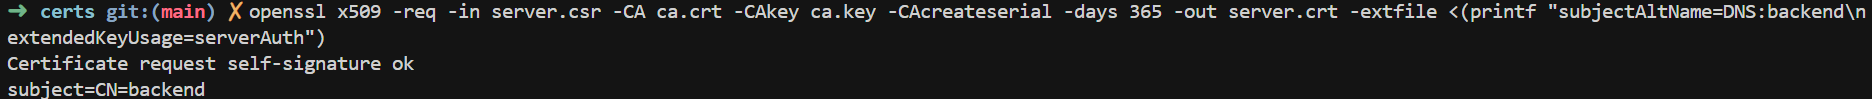
\includegraphics[width=1.1\linewidth]{img/cap05-mtls-openssl.jpg}
                    \caption{Generación de CA y certificados con OpenSSL.}
                    \label{fig:mtls-openssl}
                \end{figure}
                
                \item \textbf{Montar los certificados en runtime} — los ficheros se inyectan como volúmenes al arrancar el contenedor, no se incluyen en la imagen Docker. Así podemos rotar material criptográfico sin reconstruir la imagen (\cref{fig:mtls-volumes}).

                \begin{figure}[H]
                    \centering
                    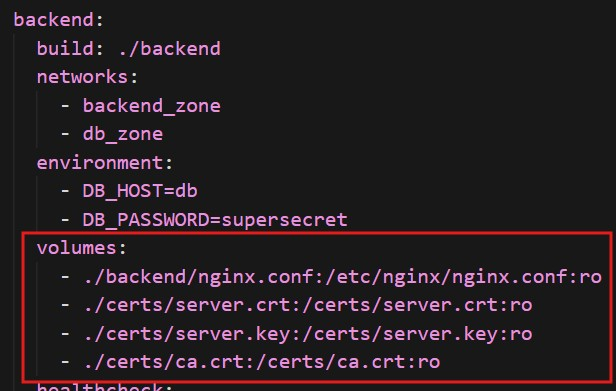
\includegraphics[width=0.6\linewidth]{img/cap05-mtls-volumes.jpg}
                    \caption{Volúmenes de certificados en el \texttt{docker-compose}.}
                    \label{fig:mtls-volumes}
                \end{figure}
                
            \end{itemize}
            
            \item A nivel de aplicación:
            \begin{itemize}
                \item \textbf{Configurar Nginx como PEP dentro de `backend`} — escucha en el puerto 443, exige certificado de cliente (`ssl\_verify\_client on`) y reenvía al proceso Flask en backend (\cref{fig:mtls-nginx-conf}).
                
                Añadimos otro nginx a backend que actúa como verificador, webapp ya no se conecta a backend directamente, sino que pasa a través de este nginx.

                \begin{figure}[H]
                    \centering
                    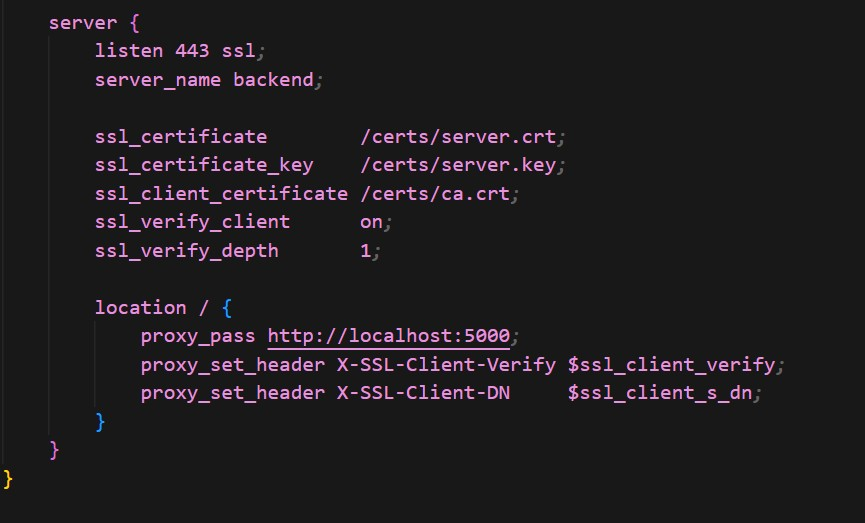
\includegraphics[width=0.6\linewidth]{img/cap05-mtls-nginx-conf.jpg}
                    \caption{\texttt{nginx.conf} del contenedor \texttt{backend} con verificación de cliente mTLS.}
                    \label{fig:mtls-nginx-conf}
                \end{figure}
                
                
                \item \textbf{Configurar el cliente en `webapp`} — las peticiones a la API usan HTTPS presentando el certificado de cliente firmado por la CA local (\cref{fig:mtls-webapp-client}).

                \begin{figure}[H]
                    \centering
                    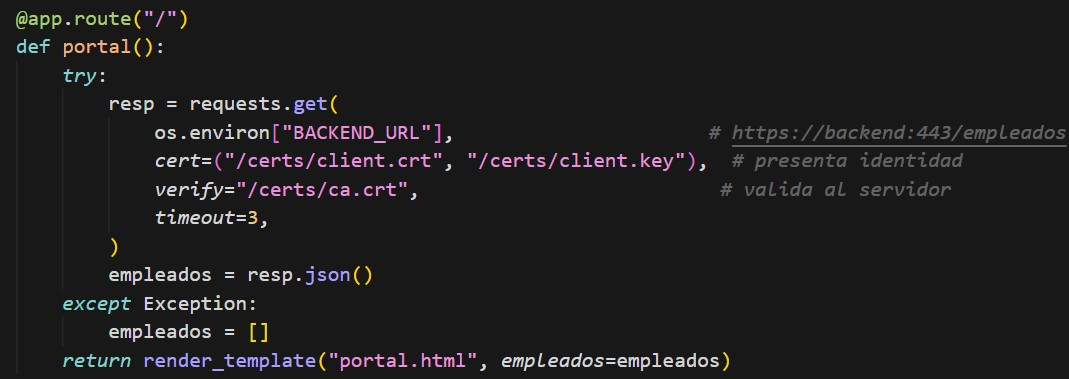
\includegraphics[width=0.85\linewidth]{img/cap05-mtls-webapp-client.jpg}
                    \caption{Cliente HTTPS/mTLS en \texttt{webapp} (\texttt{app.py}).}
                    \label{fig:mtls-webapp-client}
                \end{figure}
        
            \end{itemize}
        \end{enumerate}

        Las figuras documentan esos cuatro pasos: la emisión del material criptográfico con OpenSSL (\cref{fig:mtls-openssl}), su inyección como volúmenes de solo lectura sin reconstruir la imagen (\cref{fig:mtls-volumes}), la configuración de Nginx como verificador de cliente en \texttt{backend} (\cref{fig:mtls-nginx-conf}) y la adaptación del cliente en \texttt{webapp} para presentar su certificado (\cref{fig:mtls-webapp-client}).
        
        Para verificar la implantación ejecutamos la misma petición al backend con y sin certificado de cliente, como se aprecia en \cref{fig:mtls-verificacion}. La petición que presenta el certificado firmado por la CA obtiene una respuesta correcta (HTTP 200), mientras que la petición sin certificado es rechazada por Nginx con un error 400 antes de llegar a la aplicación. La figura evidencia así el doble papel del mTLS: cifra el canal y, además, autentica al cliente, de modo que un servicio sin identidad válida no puede consumir la API interna aunque alcance el puerto.

        \begin{figure}[ht]
            \centering
            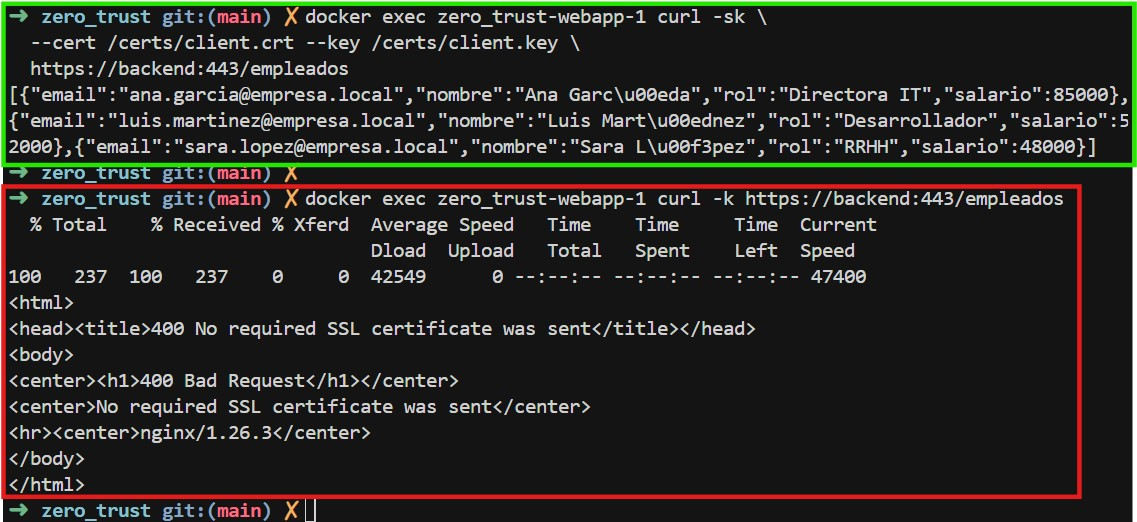
\includegraphics[width=0.85\linewidth]{img/cap05-mtls-verificacion.jpg}
            \caption{Verificación mTLS: \texttt{curl} con y sin certificado de cliente contra \texttt{backend:443}.}
            \label{fig:mtls-verificacion}
        \end{figure}
        \FloatBarrier
        
        \subsection{Desarrollo y Despliegue de Wazuh}
        \label{sec:5.3.4}

        A diferencia de los demás servicios, Wazuh no forma parte del stack de la aplicación, sino que se despliega en un segundo Docker Compose que se conecta a las redes ya creadas por el Escenario B \cite{wazuhdocs}. De este modo añadimos la observabilidad sin alterar la topología ni los contenedores que se están midiendo. El montaje siguió estos pasos:
        \begin{enumerate}
            \item \textbf{Levantar manager y agente} como contenedores adicionales vinculados a las redes del Escenario B (véase \cref{fig:wazuh-despliegue}).
            \item \textbf{Montar el socket de Docker en el agente} y arrancarlo con visibilidad de procesos del host (`--pid=host`), de modo que pueda inspeccionar los procesos que se ejecutan dentro de `webapp`.
            \item \textbf{Configurar el recolector} para que cada dos segundos ejecute un script que, a través de la API de Docker, lee `/proc/*/cmdline` dentro de `webapp` (fuente `process-webapp`).
            \item \textbf{Cargar las reglas locales} en el manager y reiniciar manager y agente para aplicar la configuración.
            \item \textbf{Comprobar el enrollment}: el agente debe aparecer activo en el manager antes de iniciar la ventana post-RCE.
        \end{enumerate}

        \begin{figure}[H]
            \centering
            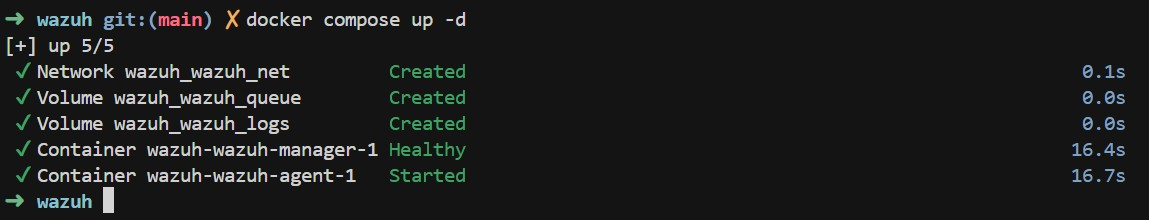
\includegraphics[width=0.85\linewidth]{img/cap05-wazuh-despliegue.jpg}
            \caption{Despliegue de Wazuh: \texttt{docker-compose}, redes externas y configuración del agente.}
            \label{fig:wazuh-despliegue}
        \end{figure}

        Sobre los eventos de `process-webapp` aplicamos reglas locales alineadas con los hitos de la cadena de ataque:

        \begin{table}[H]
          \centering
          \begin{tabular}{|c|p{9.5cm}|}
            \hline
            \textbf{Regla} & \textbf{Comportamiento detectado} \\
            \hline
            100100 & Escaneo con \texttt{nmap} \\
            \hline
            100101 & \texttt{curl} hacia \texttt{backend} \\
            \hline
            100102 & Captura con \texttt{tcpdump} \\
            \hline
            100103 & Acceso con \texttt{psql} \\
            \hline
            100104 & Búsqueda de credenciales (\texttt{grep}) \\
            \hline
          \end{tabular}
          \caption{Reglas locales Wazuh alineadas con los hitos post-explotación (\texttt{process-webapp}).}
          \label{tab:wazuh-reglas}
        \end{table}

        Un muestreo de respaldo con `process-list` cada cinco segundos cubre procesos más duraderos.

    \section{Puesta en marcha del laboratorio}
    \label{sec:5.4}
    
    Pasamos de la implantación a un laboratorio operativo siguiendo un procedimiento común para ambos escenarios, con una variante en Zero Trust por la dependencia de Wazuh respecto a las redes del stack principal.
    
    \subsubsection{Requisitos del host}
    \begin{enumerate}
        \item Docker Desktop con motor Linux (en nuestro caso sobre WSL2 en Windows).
        \item Docker Compose v2.
    \end{enumerate}
    
    \subsubsection{Puesta en marcha de ambos Escenarios}
    Gracias a la facilidad de despliegue en docker, para poner en marcha cualquiera de los dos escenarios y comprobar si lo desarrollado funciona basta con ejecutar `docker compose up --build -d`

    \begin{figure}[ht]
        \centering
        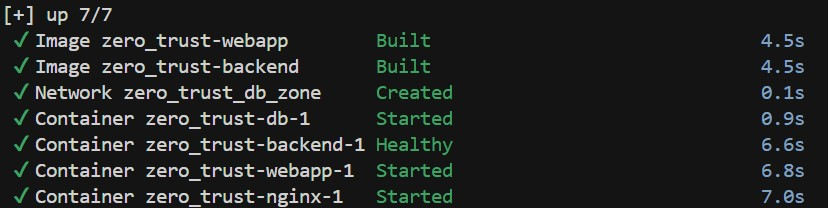
\includegraphics[width=0.85\linewidth]{img/cap05-docker-compose-up.jpg}
        \caption{Arranque del escenario con \texttt{docker compose up --build -d} y contenedores activos.}
        \label{fig:docker-compose-up}
    \end{figure}

    Una vez hecho esto veremos como se despliegan todos los contenedores especificados en el compose.    
    
    \subsubsection{Paso extra del Escenario B (Zero Trust)}
    La red Zero Trust posee algo que la red perimetral no: Wazuh.

    Antes (\cref{sec:5.3.4}) hemos mencionado que Wazuh se despliega en un docker-compose aparte y se adhiere a la red Zero Trust existente

    Esto requiere que, una vez que la red esté operativa, levantemos el compose de Wazuh con el mismo comando, esto añadirá de manera efectiva la observabilidad activa a la red zero trust. La situación de Wazuh dentro de la topología Zero Trust se representa en el diagrama de \cref{sec:4.3.4}.
    
    \subsection{Scripts de arranque}
    \label{sec:5.4.1}
    Para facilitar el despliegue del laboratorio, la realización de las pruebas y recogida de evidencias, automatizamos el despliegue y recogida de datos en ambos escenarios.

    Los scripts reciben el nombre de logcapture\_perimetral.sh y logcapture\_zerotrust.sh

    Ambos realizan las siguientes tareas:
    \begin{enumerate}
        \item Levantar el entorno con docker compose up
        \item Una vez el entorno se ha levantado sin errores, dejan una pausa para realizar las pruebas y esperan input del usuario para continuar
        \item Una vez terminada la sesión de pruebas, se copian los logs generados en webapp y se vuelcan a una carpeta en el host
    \end{enumerate}El detalle de cada script figura en el anexo \ref{anexo:scripts_captura}.
    
    \section{Problemas de integración encontrados}
    Durante la implantación aparecieron incidencias que no estaban en el diseño inicial pero condicionaron el resultado final. Documentamos las que afectaron a la reproducibilidad o a la coherencia entre diseño y realidad.
    
    \subsubsection{Artefactos de sesión vacíos.} 
    En una sesión de prueba temprana, algunos logs quedaron vacíos porque el entorno se destruyó antes de copiarlos desde el contenedor. Integramos la copia con `docker compose cp` como paso obligatorio del script, siempre anterior a un posible `compose down`.
    
    \subsubsection{Bypass del PEP por Flask en `0.0.0.0`.} 
    Con Nginx terminando TLS en 443, Flask seguía escuchando en `0.0.0.0:5000` dentro de `backend\_zone`, de modo que \texttt{curl http://backend:5000/empleados} devolvía JSON sin pasar por mTLS. Corregimos enlazando Flask solo a `127.0.0.1`. Las sesiones de prueba realizadas antes de ese cambio no son comparables en integridad del tráfico.
    
    \subsubsection{Detección Wazuh y orden de despliegue.}
    En una sesión intermedia los controles de segmentación y mTLS funcionaron correctamente, pero no se generaron alertas. Identificamos dos causas. Por un lado, el muestreo de procesos cada quince segundos no llegaba a capturar comandos efímeros como `nmap` o `curl`. Por otro, levantar el Compose de Zero Trust recreaba las redes del stack y desestabilizaba el agente cuando Wazuh arrancaba antes que la aplicación.     La solución combinó tres medidas: reducir el muestreo de `process-webapp` a dos segundos, acoplar las reglas de detección a esa fuente y fijar el orden de arranque Zero Trust → Wazuh → validación descrito en \cref{sec:5.4}.
    
%%%%%%%%%%%%%%%%%%%%%%%%%%%%%%%%%%%%%%%%%%%%%%%%%%%%%%%%%%%%%

\chapter{Pruebas y resultados}
\label{sec:6}

    \section{Metodología de pruebas}
    \label{sec:6.1}
        \subsection{Entorno de pruebas}

        Tal y como lo hemos desarrollado, cada escenario, perimetral y Zero Trust, se despliega como un stack de contenedores independiente con la misma aplicación web vulnerable, pero con una topología de red distinta. 

        El despliegue de cada entorno y la recogida estructurada de evidencias se automatizan con los scripts `logcapture\_perimetral.sh` y `logcapture\_zerotrust.sh`, ya descritos en \cref{sec:5.4} y detallados en el \ref{anexo:scripts_captura}.
        
        \subsection{Protocolo de ejecución de las pruebas}
        El protocolo de ejecución es el mismo en ambos escenarios.
        
        Para cada sesión de estudio, los scripts de arranque mencionados (\cref{sec:5.4.1}) se encargan de empezar con un entorno limpio (`docker compose up --build -d`). 
        
        A continuación reproducimos la cadena de ataque previa a la ejecución de código remota, reconocimiento, filtrado de información, login y confirmación de SSTI, hasta conseguir una reverse shell en webapp. En el instante en que esta queda operativa marcamos el inicio de la ventana de medición.
        
        A partir de esta ventana es cuando medimos siempre los mismos cuatro hitos post-explotación:
        \begin{itemize}
            \item Exfiltración de credenciales
            \item Escaneo de la red interna
            \item Acceso al back
            \item Volcado y exfiltración de información de la Base de Datos
        \end{itemize}
        
        En cada paso guardamos el output de los comandos en logs y al terminar, el script de captura vuelca esos ficheros a una carpeta de la sesión actual para analizarlos después. 
        
        Al finalizar, detenemos y eliminamos el entorno (\texttt{docker compose down}).
        
        \subsection{Definición de la ventana de medición}
        \label{sec:6.1.3}

        Tal y como dicta el \cref{sec:3.4}, fijamos el inicio de la ventana de medición en el instante en que el atacante dispone de ejecución de código remota en webapp, con una reverse shell operativa. 

        El acceso inicial se obtiene mediante una cadena de reconocimiento y explotación previa: el atacante escanea el portal e identifica rutas comunes poco protegidas , a través de las cuales localiza credenciales expuestas que reutiliza para autenticarse y, finalmente, explotar una inyección de plantillas del lado del servidor (SSTI) que le concede ejecución remota. El detalle de esta cadena se documenta en \cref{sec:5.2.3}.
        
        La fase previa al RCE sirve para narrar cómo se compromete el portal, pero no entra en el cuadro comparativo entre escenarios: el punto de entrada está fijado por diseño en ambos. A partir de este punto consideramos la "Assumed breach" y además mediremos:
        \begin{itemize}
            \item Detección
            \item Profundidad del ataque
            \item Bloqueo de comandos desde reverse shell
            \item Superficie visible
            \item Volumen exfiltrado
            \item Integridad del tráfico interno
        \end{itemize}
        
    \section{Resultados — Escenario A (Perimetral)}
    \label{sec:6.2}
    
        \subsection{Métricas KPI — Escenario A}
        \begin{table}[ht]
          \centering
          \label{tab:kpi-a}
          \small
          \begin{tabular}{p{1cm} p{8cm}}
            \textbf{Código} & \textbf{Valor} \\
            \midrule
            G1 & \texttt{(false, $\infty$)} --- sin SIEM, sin alerta \\
            G2 & 3 nodos (\texttt{webapp} $\rightarrow$ \texttt{backend} $\rightarrow$ \texttt{db}) \\
            G3 & \texttt{(false, 0\%)} --- ningún hito bloqueado \\
            E1 & 3/3 servicios visibles desde \texttt{webapp} \\
            E2 & 3 registros de empleados + 1 cred.\ DB / $\sim$766\,B \\
            E3 & Texto claro (HTTP/JSON sin TLS) \\
            \bottomrule
          \end{tabular}
          \caption{Métricas KPI — Escenario A (Perimetral).}
        \end{table}

        En el escenario perimetral no hay ningún sistema de detección activo (G1): los accesos quedan solo en logs pasivos de nginx y webapp, sin alertas ni correlación de eventos.

        Una vez dentro de webapp, el atacante consigue proyectarse hasta el backend y la base de datos (G2): la brecha alcanza los tres nodos del stack sin que ningún control de segmentación lo impida.
        
        Ningún mecanismo de bloqueo actúa sobre el movimiento lateral (G3): la exfiltración de credenciales, las peticiones al API interno y la consulta SQL terminan con éxito.
        
        Desde webapp el escaneo interno muestra los tres servicios (E1), backend en el puerto 5000, la base de datos en el 5432 y nginx en el 80, con total visibilidad de la red plana (\cref{fig:nmap-perimetral}).
        \begin{figure}[H]
            \centering
            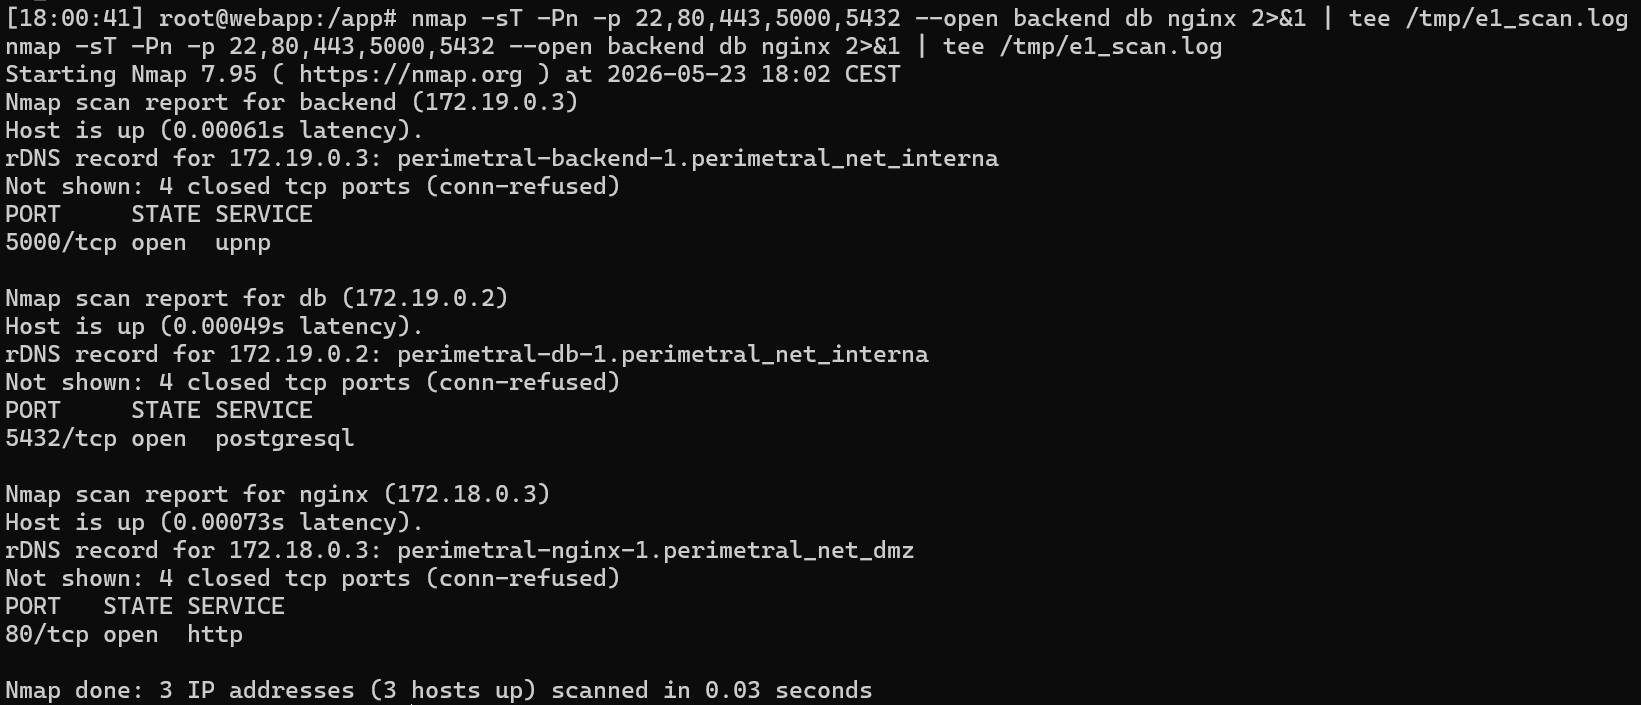
\includegraphics[width=0.9\linewidth]{img/cap06-nmap-perimetral.jpg}
            \caption{Escaneo \texttt{nmap} interno desde \texttt{webapp} en el Escenario A.}
            \label{fig:nmap-perimetral}
        \end{figure}
        
        La exfiltración es efectiva (E2): obtiene la contraseña de la BD del entorno del contenedor, descarga el JSON de tres empleados desde `/empleados` y vuelca la tabla completa, unos 766 bytes entre credenciales y datos (\cref{fig:exfil-empleados}, \cref{fig:exfil-sql}).
        \begin{figure}[ht]
            \centering
            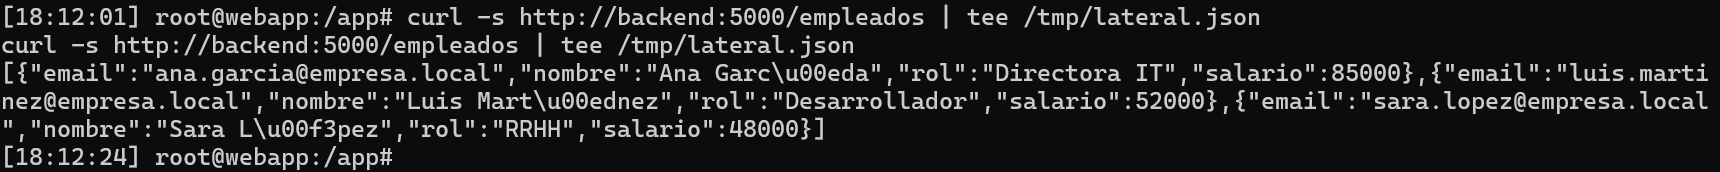
\includegraphics[width=1\linewidth]{img/cap06-exfil-empleados.jpg}
            \caption{Petición a \texttt{/empleados} y JSON de empleados exfiltrado (Escenario A).}
            \label{fig:exfil-empleados}
        \end{figure}

        \begin{figure}[ht]
            \centering
            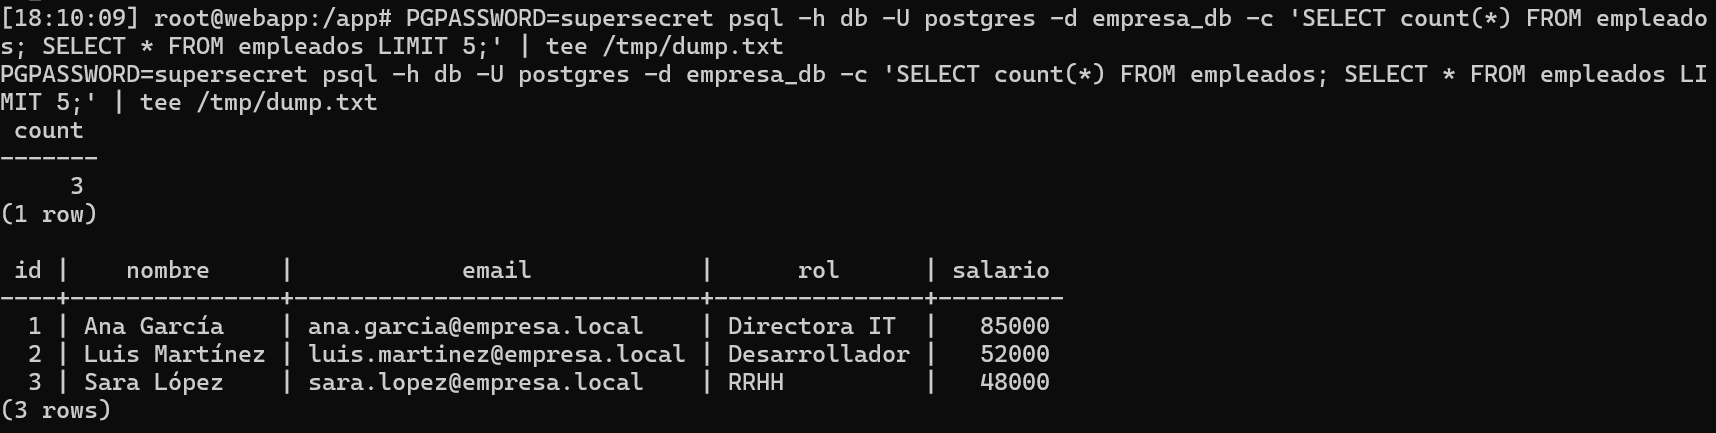
\includegraphics[width=0.9\linewidth]{img/cap06-exfil-sql.jpg}
            \caption{Consulta SQL y volcado de la base de datos (Escenario A).}
            \label{fig:exfil-sql}
        \end{figure}
        
        Como el tráfico entre contenedores no va cifrado (E3), puede capturar el intercambio HTTP con tcpdump y leer el JSON en claro en el pcap (\cref{fig:tcpdump-pcap}).

        \begin{figure}[ht]
            \centering
            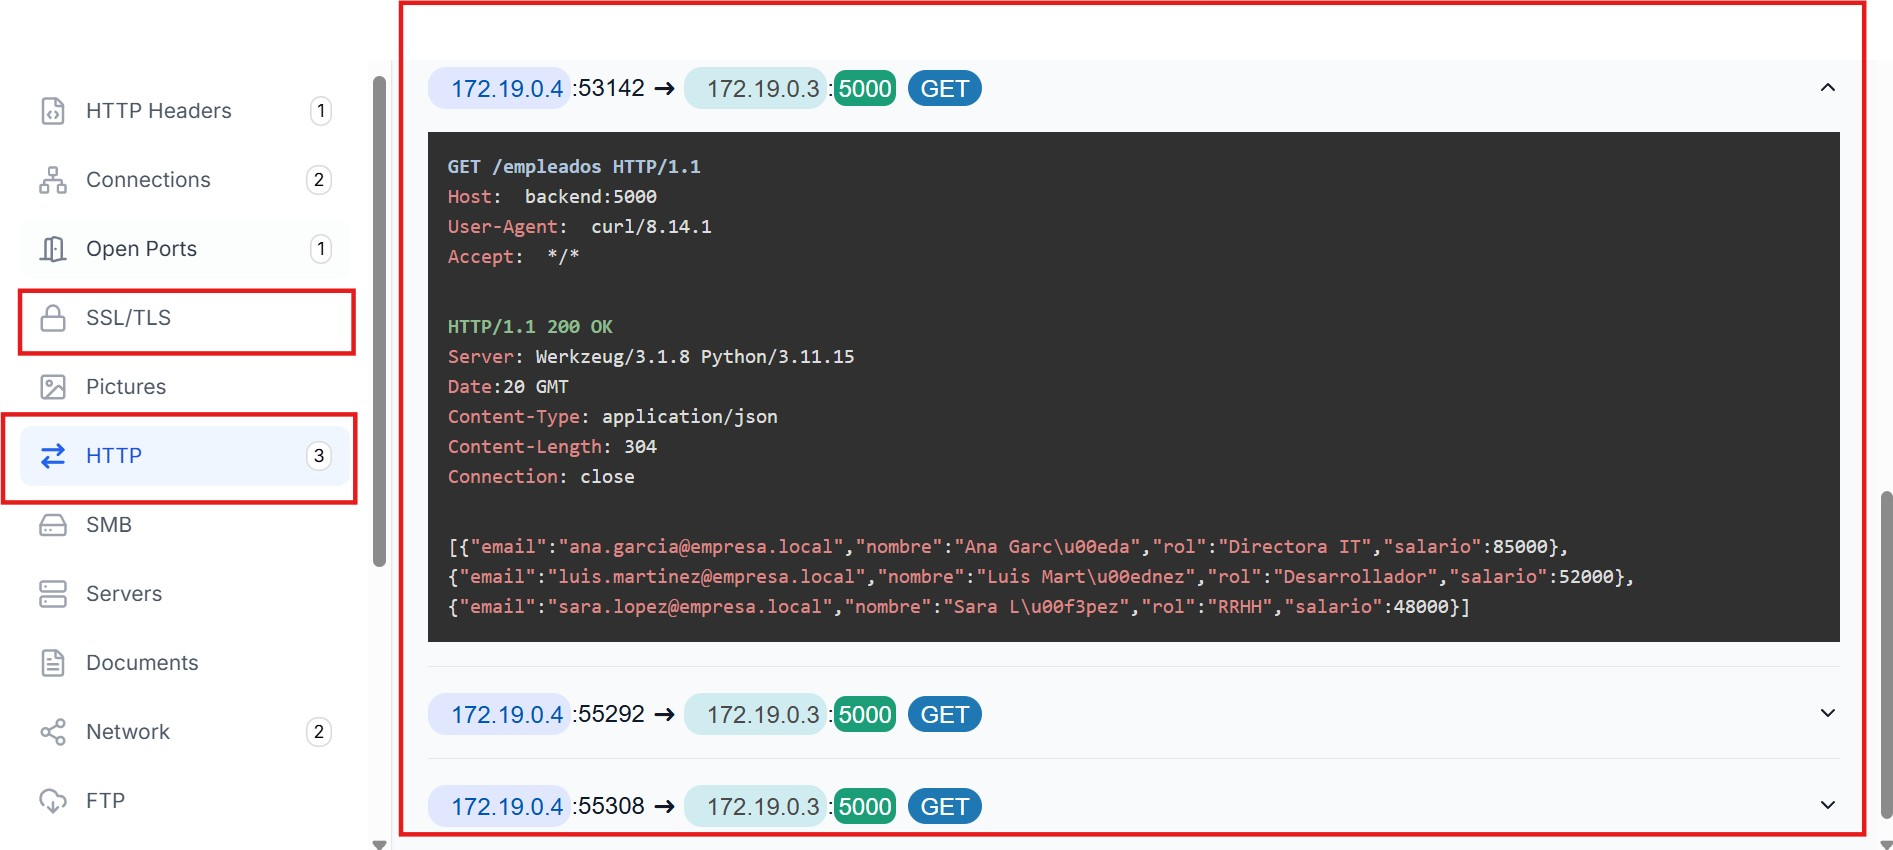
\includegraphics[width=0.9\linewidth]{img/cap06-tcpdump-pcap.jpg}
            \caption{Captura \texttt{tcpdump} y tráfico HTTP en claro en el pcap (Escenario A).}
            \label{fig:tcpdump-pcap}
        \end{figure}
        \FloatBarrier
        
    \section{Resultados — Escenario B (Zero Trust)}
        
        \subsection{Métricas KPI — Escenario B}
        \begin{table}[ht]
          \centering
          \label{tab:kpi-b}
          \footnotesize
          \begin{tabular}{p{1cm} p{12cm}}
            \textbf{Código} & \textbf{Valor} \\
            \midrule
            G1 & \texttt{(true, 22\,s)} --- 1.\textsuperscript{a} alerta Wazuh regla \textbf{100100} (nmap) a 22s de inicio \\
            G2 & \textbf{1 nodo}: \texttt{webapp} $\checkmark$ --- \texttt{backend} $\times$ --- \texttt{db} $\times$ \\
            G3 & \texttt{(true, 100\,\%)} --- exfiltración, movimiento lateral y acceso a DB fallaron, con JSON cifrado \\
            E1 & \textbf{1 / 3} --- \texttt{nginx:80} y \texttt{backend:443} visibles; \texttt{db} no resuelve; \texttt{:5000} cerrado \\
            E2 & \textbf{0 registros / 0\,B} --- sin credenciales en env ni JSON de empleados \\
            E3 & \textbf{cifrado + rechazado} \\
            \bottomrule
          \end{tabular}
          \caption{Métricas KPI — Escenario B (Zero Trust).}
        \end{table}

        Los seis indicadores traducen la cronología anterior a magnitudes comparables (\cref{sec:3.4}).
        
        La primera alerta de Wazuh (G1) llega 22 segundos después del inicio de la ventana de medición, asociada al escaneo nmap de reconocimiento interno y a la regla local correspondiente (\cref{tab:wazuh-reglas}, regla 100100; \cref{lst:wazuh-nmap-zt}).

        \begin{lstlisting}[
            caption={Alerta Wazuh regla 100100 tras escaneo \texttt{nmap} post-RCE (Escenario B).},
            label={lst:wazuh-nmap-zt},
            basicstyle=\ttfamily\footnotesize,
            breaklines=true
        ]
{"timestamp":"2026-06-09T11:16:37.276+0000","rule":{"level":12,"description":"ZT (webapp): nmap post-RCE - reconocimiento interno (T1046)","id":"100100","firedtimes":5,"mail":true,"groups":["zerotrust"]},"agent":{"id":"001","name":"zt-lab-agent","ip":"172.21.0.3"},"manager":{"name":"wazuh-manager"},"id":"1781003797.760441","full_log":"ossec: output: 'process-webapp': nmap -sT -Pn -p 5432 db ","decoder":{"name":"ossec"},"location":"process-webapp"}
        \end{lstlisting}
        
        La profundidad del ataque (G2) se reduce a un nodo, `webapp`: ni el backend ni la base de datos llegan a ser operativos para el ataque, porque el primero rechaza las peticiones sin certificado de cliente y la segunda no es siquiera alcanzable. La brecha persiste en el nodo de entrada pero no se propaga: el atacante conserva la reverse shell, sin convertir esa posición en alcance sobre la infraestructura.
        
        La tasa de bloqueo (G3) cubre los tres hitos post-explotación dirigidos contra activos protegidos: exfiltración de credenciales, acceso a la API del backend y volcado de la base de datos. Los tres quedan frustrados, cada uno por un control distinto, aislamiento de secretos, autenticación mutua y segmentación, lo que muestra que la contención no descansa en una única barrera. El único hito que devuelve información al atacante es el escaneo interno, que no constituye acceso a un activo y solo confirma la reducción de superficie accesible que mide E1.
        
        El escaneo interno (E1) identifica con utilidad únicamente nginx en el puerto 80 y el puerto 5000 del backend aparece cerrado. La base de datos no solo no resuelve por DNS: como `webapp` no comparte ninguna red con `db\_zone`, tampoco es alcanzable por su dirección IP directa, de modo que la microsegmentación elimina la ruta a nivel de red y no solo la resolución de nombres. El backend responde en el 443, pero ese puerto está protegido por mTLS y no es superficie aprovechable. El activo principal desaparece del mapa que el atacante puede construir desde el nodo comprometido (\cref{fig:nmap-zerotrust}).

        \begin{figure}[ht]
            \centering
            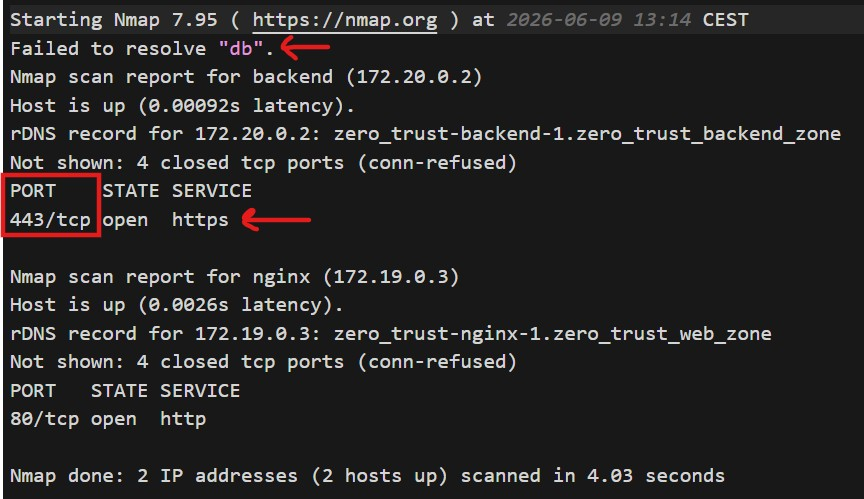
\includegraphics[width=0.85\linewidth]{img/cap06-nmap-zerotrust.jpg}
            \caption{Escaneo \texttt{nmap} interno desde \texttt{webapp} en el Escenario B.}
            \label{fig:nmap-zerotrust}
        \end{figure}

        La exfiltración de credenciales falla (E2): el entorno de \texttt{webapp} no contiene \texttt{DB\_PASSWORD} ni \texttt{DB\_HOST}, y el fichero \texttt{creds.txt} que el script de captura vuelca tras la sesión (\cref{sec:6.1}) queda vacío. Pese a mantenerse la ejecución remota en \texttt{webapp}, la intrusión no extrae secretos de base de datos.

        El intento de movimiento lateral hacia la API del backend se frustra (G3): el puerto 5000 rechaza la conexión y la petición HTTPS a \texttt{/empleados} devuelve 400 por falta de certificado de cliente (\cref{fig:mtls-verificacion}); \texttt{lateral.json} queda vacío.

        El volcado de la base de datos no es posible: como ya indica el escaneo interno (\cref{fig:nmap-zerotrust}), \texttt{db} no resuelve por DNS desde \texttt{webapp}, y \texttt{psql} falla al intentar conectar.

        La captura de tráfico generada por el propio atacante (E3) ---log \texttt{lateral.pcap}, 26 paquetes--- contiene únicamente tráfico TLS, por lo que la interceptación no recupera contenido útil (\cref{fig:tcpdump-zt}). El rechazo en el backend confirma el doble papel del mTLS descrito en \cref{sec:5.3.3}.

        \begin{figure}[ht]
            \centering
            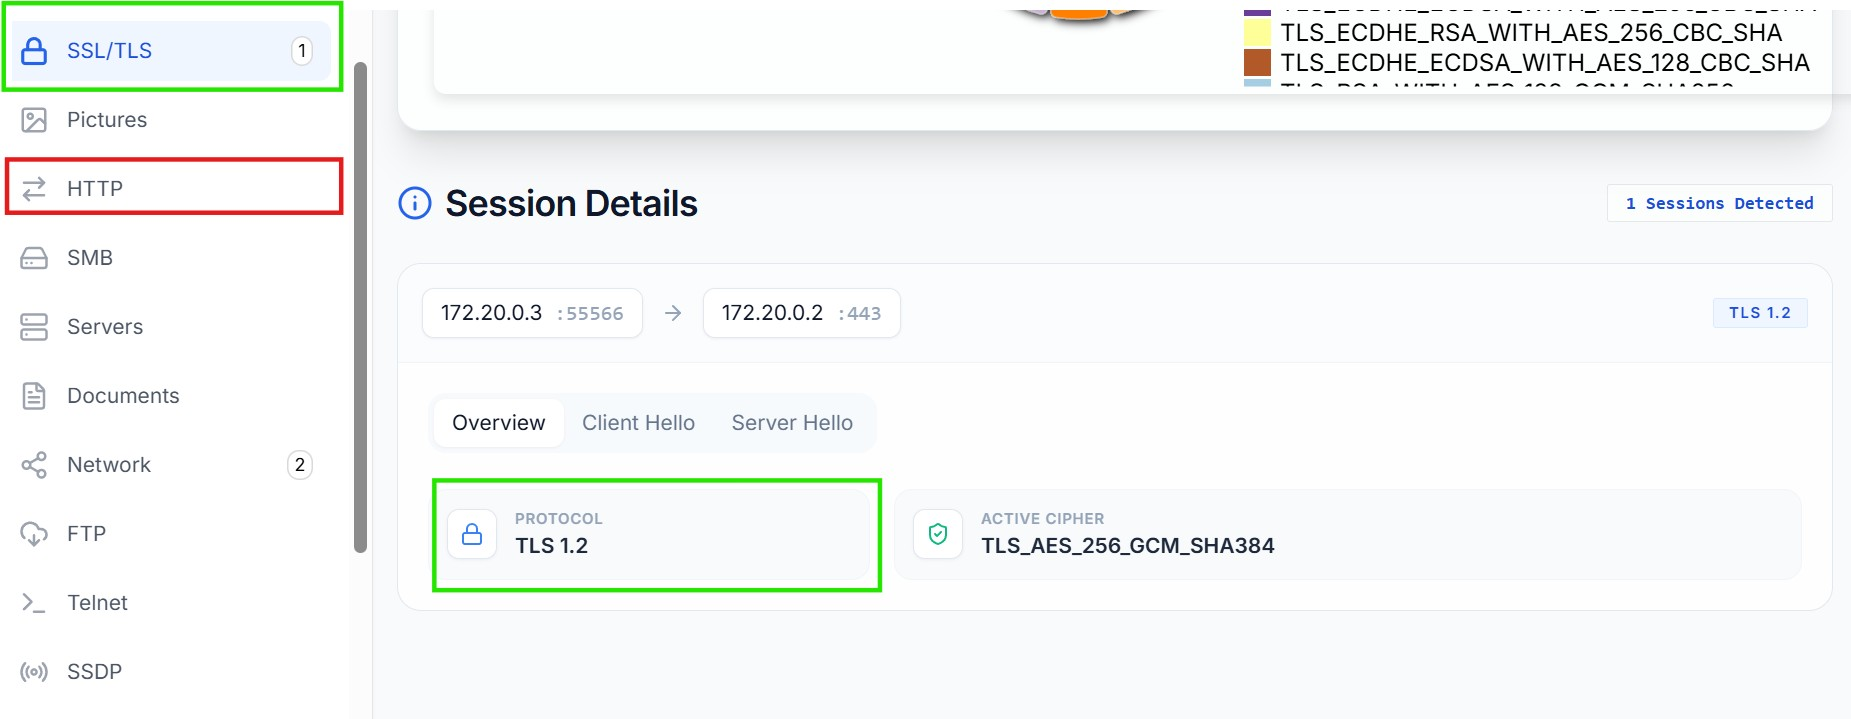
\includegraphics[width=0.9\linewidth]{img/cap06-tcpdump-zt.jpg}
            \caption{Captura \texttt{tcpdump} con tráfico TLS sin JSON en claro (Escenario B).}
            \label{fig:tcpdump-zt}
        \end{figure}
        \FloatBarrier

    \section{Comparativa Perimetral vs Zero Trust}
    \label{sec:6.4}
        \subsection{Tabla comparativa final}
        \begin{table}[ht]
          \centering
          \label{tab:comparativa-ab}
          \footnotesize
          \begin{tabularx}{\textwidth}{@{}>{\raggedright\arraybackslash}p{3.2cm} X X X@{}}
            \toprule
            \textbf{Indicador} & \textbf{Escenario A} & \textbf{Escenario B} & \textbf{Mejora observada} \\
            \midrule
            Detección (G1) & \texttt{(false, $\infty$)} & \texttt{(true, 22\,s)} & El nmap se detecta gracias a la observación activa \\
            Profundidad del ataque (G2) & 3 nodos & 1 nodo & $-$67\,\% alcance lateral (2 nodos menos) \\
            Bloqueo de comandos desde reverse shell (G3) & \texttt{(false, 0\,\%)} & \texttt{(true, 100\,\%)} & De contención inexistente a bloquear comandos post-explotación \\
            Superficie visible (E1) & 3/3 servicios & 1/3 & $-$67\,\% superficie visible (\texttt{db} no resuelve; \texttt{:5000} cerrado) \\
            Volumen exfiltrado (E2) & $\sim$766\,B / 3 reg.\ + 1 cred. & 0\,B / 0 reg. & Exfiltración anulada \\
            Integridad del tráfico interno (E3) & Texto claro (HTTP) & Cifrado + rechazado & mTLS + PEP (400 sin certificado cliente) \\
            \bottomrule
          \end{tabularx}
          \caption{Comparativa de indicadores — Escenario A vs Escenario B.}
        \end{table}

        La tabla anterior condensa lo medido en la fase post-explotación, a partir de los mismos cuatro hitos en ambos escenarios (véase \cref{sec:6.1.3}). 

        Con estos seis indicadores respondemos, con datos reproducibles, en qué medida la arquitectura Zero Trust reduce el impacto frente al modelo perimetral en:
        \begin{itemize}
            \item Detección
            \item Profundidad del ataque
            \item Bloqueo de comandos desde reverse shell
            \item Superficie visible
            \item Volumen exfiltrado
            \item Integridad del tráfico interno
        \end{itemize}
        
        En el escenario perimetral el atacante recorre los tres nodos de la red sin que ningún control lo detenga. En cambio, en Zero Trust el compromiso queda acotado a webapp y Wazuh registra actividad. 
        
        El desglose por dimensión y la atribución de cada mecanismo están en \cref{sec:6.4.2}; los matices de interpretación, en \cref{sec:6.4.3}.
        
        \subsection{Análisis de la mejora}
        \label{sec:6.4.2}

        Las dos secciones anteriores presentan los valores de cada escenario por separado; aquí los contrastamos dimensión a dimensión para atribuir cada mejora al mecanismo concreto que la produce.

        En detección, el escenario perimetral no dispone de mecanismo activo: solo quedan logs pasivos de nginx y webapp, sin alertas. Zero Trust introduce Wazuh, que muestrea cada 2 segundos los procesos en webapp; la primera alerta llega asociada al escaneo nmap.

        La profundidad del ataque pasa de tres nodos a uno: una reducción del 67\% en alcance lateral. La microsegmentación en tres zonas impide que webapp alcance `db\_zone`, Flask escucha solo en `127.0.0.1` dentro del backend y el atacante no consigue operar con utilidad en backend ni en la base de datos, aunque mantenga la reverse shell en webapp.
        
        El bloqueo de comandos desde reverse shell refleja el mismo contraste: en A ningún objetivo post-explotación falla al ejecutarse desde la shell. En B los tres quedan frustrados:
        \begin{enumerate}
            \item Los secretos de base de datos viven solo en backend.
            \item El canal hacia la API exige certificado de servicio.
            \item La segmentación corta el acceso directo a la base de datos.
        \end{enumerate}
        
        La superficie visible interna se reduce de tres servicios accesibles a uno de tres: `db` no resuelve por DNS desde webapp y el puerto 5000 del backend aparece cerrado. El escaneo desde el nodo comprometido solo identifica nginx en el 80 y el backend en el 443, frente a la visibilidad total de la red interna en el escenario perimetral.
        
        En exfiltración, el volumen fugado cae de unos 766 bytes (tres registros de empleados, la contraseña de la base de datos y el JSON de la API) a cero. Sin credenciales en el entorno de webapp y sin respuesta útil del backend, los logs que evidencian el volumen de datos exfiltrados quedan vacíos en la sesión Zero Trust.
        
        En integridad del tráfico, el contraste es cualitativo pero contundente:
        \begin{enumerate}
            \item En el escenario perimetral, el pcap muestra HTTP y JSON en claro.
            \item En Zero Trust, el tráfico hacia backend va cifrado con TLS y, sin certificado cliente, nginx devuelve error 400.
        \end{enumerate}
        
        El atacante no puede replicar la lectura pasiva del intercambio que sí logró en el escenario perimetral.
        
        En conjunto, estos resultados cuantifican un patrón que la literatura revisada en \cref{sec:2.4} apenas aborda con métricas comparables.

        \subsection{Matices de la interpretación}
        \label{sec:6.4.3}

        En profundidad del ataque, bloqueo de comandos, superficie visible, exfiltración e integridad del tráfico no observamos ningún empeoramiento respecto al modelo perimetral: Zero Trust reduce o anula el impacto post-explotación en todas estas dimensiones. 
        
        El único matiz está en la detección. En el Escenario A no existe SIEM por diseño, de modo que comparar la latencia de la primera alerta no constituye un contraste equitativo; lo que la tabla acredita no es que el Escenario B detecte «antes», sino que la capacidad de detección activa existe únicamente en la arquitectura Zero Trust.

%%%%%%%%%%%%%%%%%%%%%%%%%%%%%%%%%%%%%%%%%%%%%%%%%%%%%%%%%%%%%%%%%%%%%%%%%%%%%%%
%                                 CONCLUSIONS                                 %
%%%%%%%%%%%%%%%%%%%%%%%%%%%%%%%%%%%%%%%%%%%%%%%%%%%%%%%%%%%%%%%%%%%%%%%%%%%%%%%

\chapter{Conclusiones}

        \section{Conclusiones del estudio}
        Este trabajo se planteó para responder a una pregunta concreta:

        \begin{tcolorbox}[
            enhanced,
            frame hidden,
            borderline west={3pt}{0pt}{gray!70!black},
            sharp corners
        ]
            ¿En qué medida aplicar la metodología Zero Trust reduce el impacto de ataques post-explotación frente a un modelo perimetral, y cómo lo hace esto superior?
        \end{tcolorbox}

        A partir de la evidencia recogida en la sesión oficial de cada escenario (\cref{sec:6.4}), la respuesta es que la reducción es sustancial en casi todas las dimensiones medidas: partiendo del mismo compromiso inicial, una ejecución remota de código en el servicio web, el modelo perimetral permitió al atacante alcanzar los tres nodos de la red y extraer información, mientras que el modelo Zero Trust confinó el compromiso al nodo de entrada e impidió que los hitos post-explotación prosperaran.

        La hipótesis de partida (\cref{sec:1.2}) se confirma en lo esencial. Los tres efectos previstos, menor profundidad del compromiso, menor volumen de datos exfiltrados y mayor protección del tráfico interno, se observan con claridad: la profundidad del ataque se redujo de tres nodos a uno, la exfiltración pasó de varios cientos de bytes a cero y el tráfico interno dejó de ser legible al exigirse autenticación mutua. El único matiz afecta a la detección: al no existir SIEM en el Escenario A por diseño, su comparación con el Escenario B no es equitativa, según se detalla en \cref{sec:6.4.3}.

        Más allá de esos tres efectos, la adición de observabilidad activa, aunque implementada de una forma básica, ofrece un punto de calidad extra a la hora de gestionar la seguridad de una red.

        En cuanto a los objetivos específicos planteados en \cref{sec:1.2}, los cuatro se alcanzaron. Se diseñaron y desplegaron dos infraestructuras funcionalmente idénticas que solo difieren en su modelo de red (objetivo primero, desarrollado en \cref{sec:4}). Se definió y midió un conjunto de métricas de contención y detección estrictamente comparables entre ambos escenarios (objetivo segundo, \cref{sec:3.4} y \cref{sec:6}). Se ejecutó el mismo protocolo de ataque post-explotación de forma reproducible en los dos entornos (objetivo tercero, \cref{sec:6.1}). Y se cuantificó el impacto de la microsegmentación y la observabilidad sobre la capacidad de contención (objetivo cuarto).

        El análisis por indicadores permite atribuir cada mejora a un mecanismo concreto. 
        \begin{enumerate}
            \item La reducción de la profundidad del ataque y de la superficie interna visible es consecuencia directa de la microsegmentación en tres zonas y de la decisión de que el backend escuche solo en su interfaz de loopback: el atacante conserva la shell en el nodo de entrada, pero no encuentra rutas útiles hacia la base de datos. 
            \item El bloqueo de los comandos post-explotación combina tres controles: 
                \begin{itemize}
                    \item La separación de secretos por servicio
                    \item La autenticación mutua en el canal hacia el backend 
                    \item La propia segmentación
                \end{itemize}
                De modo que ninguno de los objetivos del atacante sobre los activos protegidos llega a completarse. De ahí se derivan también la anulación de la exfiltración y la protección del tráfico.
        \end{enumerate}
        En conjunto, el estudio respalda que una arquitectura Zero Trust basada en microsegmentación e identidad de servicio reduce de forma significativa el impacto de una intrusión post-explotación en una infraestructura contenerizada.

        \section{Limitaciones del trabajo}
        \label{sec:7.2}
        Las conclusiones anteriores deben leerse a la luz de varias limitaciones que acotan su validez.

        La principal es el tamaño de la muestra. Los valores comparados proceden de una única sesión oficial por escenario, son reproducibles mediante los scripts de captura y coherentes con el comportamiento esperado de cada control, pero no constituyen una estimación estadística con intervalos de confianza. Las cifras concretas, la reducción de la profundidad o de la superficie visible, el porcentaje de bloqueo, deben interpretarse como ilustrativas del comportamiento de cada arquitectura, no como medias de una población de ensayos.

        El alcance del experimento es la segunda limitación. El estudio parte de un atacante que ya dispone de ejecución remota de código en el servicio web: no evalúa cómo se previene el compromiso inicial, sino qué ocurre después. Esta delimitación es deliberada y coherente con el modelo de amenazas (\cref{sec:3.2}), pero implica que las conclusiones se refieren a la contención del daño post-explotación y no a la seguridad del sistema en su conjunto.

        A ello se suman las limitaciones de diseño ya expuestas en \cref{sec:4.5}, que también condicionan la generalización de los resultados: el mTLS protege un único canal, la observabilidad se despliega sin respuesta automatizada y el entorno es un laboratorio local sobre Docker, no un clúster en producción.

        %[REVISADO: Ver si borramos esto, no interesas y no es tan relevante para el resultado del trabajo]
        % [Comentado y obviado de la memoria final] 
        
        %Por último, la cobertura de detección resultó parcial. El bloqueo de los hitos fue completo, pero el mecanismo de observabilidad no registró la totalidad de las acciones del atacante: las de muy corta duración pudieron transcurrir entre dos muestreos consecutivos. Esto no afecta a la contención —que depende de los controles de red e identidad—, pero sí matiza cualquier afirmación sobre la capacidad de detección del sistema.

        \section{Trabajo futuro}
        Las limitaciones anteriores señalan de forma natural las líneas de trabajo futuro más relevantes.

        La validez externa de los resultados se reforzaría llevando el experimento a un orquestador real: reimplementar las mismas políticas con NetworkPolicies de Kubernetes y un service mesh (Istio/Envoy) permitiría comprobar si la contención observada se mantiene a escala y en un entorno cloud, más cercano a producción.
        
        La protección del tráfico interno, hoy limitada a un único canal, debería extenderse a toda la malla de servicios e incorporar rotación automática de certificados, de modo que la identidad de servicio deje de ser una excepción y pase a ser la norma del sistema.

        %[REVISADO: Borrar este párrafo si borras lo de wazuh]
        % [Comentado y obviado de la memoria final]
        
        %La cobertura de detección parcial justifica añadir una capa de detección a nivel de red, como Suricata, que complemente a la detección basada en host: los ataques que evadan el muestreo de procesos podrían detectarse entonces por sus patrones de tráfico.
        
        El carácter pasivo de las alertas invita a incorporar respuesta automatizada (SOAR): vincular la detección de un hito post-explotación con una acción de contención (aislar el contenedor o cortar la conexión) cerraría el ciclo entre detectar y responder.
        
        Por último, sería valioso ampliar el repertorio de ataques: envenenamiento de DNS interno, escalada de privilegios en el host o denegación de servicio interna, y repetir el estudio con varias sesiones por escenario, lo que daría soporte estadístico a las cifras y reduciría la principal limitación del trabajo actual.

        \section{Relación con los estudios cursados}
        El desarrollo de este trabajo puso en juego buena parte de los conocimientos adquiridos durante el Grado, integrados en torno a un problema concreto. 

        Los fundamentos de redes y seguridad fueron el eje: la contraposición entre el modelo perimetral y Zero Trust, la microsegmentación y la autenticación mutua con certificados parten directamente de esos contenidos. 
        
        El diseño del laboratorio se apoyó en lo aprendido sobre sistemas distribuidos e infraestructuras.
        
        La puesta en marcha exigió nociones de administración de sistemas y de sistemas operativos, espacios de nombres, procesos, sockets y la ejecución sobre WSL2, y todo el trabajo se ordenó con prácticas de ingeniería del software: especificación de requisitos, diseño previo, infraestructura como código y reproducibilidad.
        
        Junto a lo anterior, el trabajo obligó a aprender tecnologías y conceptos que no forman parte del plan de estudios, o que solo se tratan de forma tangencial. Hubo que familiarizarse con un sistema de detección basado en host (Wazuh) y la escritura de sus reglas, con la generación y el uso de certificados para mTLS mediante OpenSSL, con la explotación de inyección de plantillas del lado del servidor (SSTI) como vector de acceso inicial y con los marcos de clasificación de amenazas como MITRE ATT\&CK. El grado de dominio alcanzado fue suficiente para diseñar, desplegar y validar los controles.
        
        Por último, el trabajo desarrolló competencias transversales relevantes: 
        \begin{itemize}
            \item El análisis crítico de los resultados sin sobrevalorarlos
            \item La comunicación escrita de un problema técnico para un lector no especialista
            \item La planificación y gestión del tiempo en sprints con plazos ajustados
        \end{itemize}

        \section{Impacto y relación con los ODS}
        
        Más allá del ejercicio académico, el trabajo aporta un criterio cuantitativo allí donde suele haber recomendaciones genéricas. Para los equipos de plataforma y de seguridad operativa, mostrar con datos cuánto se reduce el alcance de una intrusión al introducir microsegmentación e identidad de servicio ofrece un argumento concreto con el que priorizar esas inversiones. Para las organizaciones que mantienen despliegues contenerizados sobre redes planas heredadas, el estudio evidencia el riesgo real al que se exponen una vez comprometido un servicio y el grado de contención que pueden alcanzar con controles asumibles.

        Esta aportación conecta con dos Objetivos de Desarrollo Sostenible\footnote{\url{https://www.un.org/sustainabledevelopment/es/objetivos-de-desarrollo-sostenible/}}: 
        \begin{itemize}
            \item  Con el ODS 9, en tanto que contribuye a infraestructuras digitales más resilientes frente a incidentes: una red que contiene el movimiento lateral se degrada de forma controlada en lugar de comprometerse por completo.
            \item Con el ODS 16, porque reducir el impacto de las intrusiones, limita el daño que la ciberdelincuencia causa sobre ciudadanos e instituciones.
        \end{itemize}

%%%%%%%%%%%%%%%%%%%%%%%%%%%%%%%%%%%%%%%%%%%%%%%%%%%%%%%%%%%%%%%%%%%%%%%%%%%%%%%
%                                BIBLIOGRAFIA                                 %
%%%%%%%%%%%%%%%%%%%%%%%%%%%%%%%%%%%%%%%%%%%%%%%%%%%%%%%%%%%%%%%%%%%%%%%%%%%%%%%

\begin{thebibliography}{10}

% Referencias en orden de aparición. Formato orientativo ISO 690 (numérico).

\bibitem{costdatabreach}
   IBM Security; Ponemon Institute.
   \newblock \textit{Cost of a Data Breach Report 2024}.
   \newblock IBM, 2024.
   \newblock \url{https://www.ibm.com/reports/data-breach}.

\bibitem{perimetro}
   Scarfone, K.; Hoffman, P.
   \newblock \textit{Guidelines on Firewalls and Firewall Policy}.
   \newblock NIST Special Publication 800-41 Revision 1. Gaithersburg (MD):
   National Institute of Standards and Technology, 2009.
   \newblock \url{https://doi.org/10.6028/NIST.SP.800-41r1}.

\bibitem{breaches2025}
   Verizon.
   \newblock \textit{2025 Data Breach Investigations Report (DBIR)}.
   \newblock Verizon Business, 2025.
   \newblock \url{https://www.verizon.com/business/resources/reports/dbir/}.

\bibitem{kindervag2010}
   Kindervag, J.
   \newblock \textit{No More Chewy Centers: Introducing The Zero Trust Model
   Of Information Security}.
   \newblock Forrester Research, 2010.

\bibitem{nist800207}
   Rose, S.; Borchert, O.; Mitchell, S.; Connelly, S.
   \newblock \textit{Zero Trust Architecture}.
   \newblock NIST Special Publication 800-207. Gaithersburg (MD): National
   Institute of Standards and Technology, 2020.
   \newblock \url{https://doi.org/10.6028/NIST.SP.800-207}.

\bibitem{beyondcorp}
   Ward, R.; Beyer, B.
   \newblock BeyondCorp: A New Approach to Enterprise Security.
   \newblock \textit{;login:}, vol. 39, núm. 6, pp. 6--11, 2014.

\bibitem{mitrecontainers}
   The MITRE Corporation.
   \newblock \textit{ATT\&CK Matrix for Containers}.
   \newblock 2021.
   \newblock \url{https://attack.mitre.org/matrices/enterprise/containers/}.

\bibitem{jimenez2025}
   Jiménez Díaz-Varela, Mª de las Mercedes.
   \newblock \textit{Implementación de un modelo Zero Trust en un entorno Cloud
   Híbrido Simulado}.
   \newblock Trabajo Fin de Grado. Escuela Técnica Superior de Ingenieros
   Informáticos, Universidad Politécnica de Madrid, julio 2025.

\bibitem{perezg6508}
   Pérez Pérez, Gabriel.
   \newblock \textit{Zero Trust como Concepto de Seguridad}.
   \newblock Trabajo Fin de Grado. Escuela de Ingeniería Informática,
   Universidad de Valladolid, 2023.

\bibitem{torregrosa2025}
   Torregrosa Navarrete, Carlos.
   \newblock \textit{Problemática de la gestión del acceso local a redes
   corporativas y su resolución en base a sistemas NAC}.
   \newblock Trabajo Fin de Grado. Escuela Técnica Superior de Ingeniería
   Informática, Universitat Politècnica de València, curso 2024/2025.

\bibitem{vico2025}
   Vico Burruezo, Mireia.
   \newblock \textit{Implementación de un SIEM QRadar con la integración de
   Wazuh, Suricata y PFsense}.
   \newblock Trabajo Fin de Máster. Máster Universitario en Ciberseguridad y
   Ciberinteligencia, Universitat Politècnica de València, curso 2024/2025.

\bibitem{dockernet}
   Docker, Inc.
   \newblock \textit{Networking overview}.
   \newblock Docker Documentation.
   \newblock \url{https://docs.docker.com/network/}.

\bibitem{owasptop10}
   OWASP Foundation.
   \newblock \textit{OWASP Top 10:2021}.
   \newblock 2021.
   \newblock \url{https://owasp.org/Top10/}.

\bibitem{owaspssti}
   OWASP Foundation.
   \newblock \textit{Server-Side Template Injection}.
   \newblock OWASP Web Security Testing Guide.
   \newblock \url{https://owasp.org/www-community/attacks/Server_Side_Template_Injection}.

\bibitem{cwe1336}
   The MITRE Corporation.
   \newblock \textit{CWE-1336: Improper Neutralization of Special Elements Used
   in a Template Engine}.
   \newblock Common Weakness Enumeration.
   \newblock \url{https://cwe.mitre.org/data/definitions/1336.html}.

\bibitem{wazuhdocs}
   Wazuh, Inc.
   \newblock \textit{Wazuh Documentation — Deploying a Wazuh agent on Docker}.
   \newblock \url{https://documentation.wazuh.com/}.

\end{thebibliography}
\cleardoublepage

%%%%%%%%%%%%%%%%%%%%%%%%%%%%%%%%%%%%%%%%%%%%%%%%%%%%%%%%%%%%%%%%%%%%%%%%%%%%%%%
%                           APÈNDIXS  (Si n'hi ha!)                           %
%%%%%%%%%%%%%%%%%%%%%%%%%%%%%%%%%%%%%%%%%%%%%%%%%%%%%%%%%%%%%%%%%%%%%%%%%%%%%%%

\APPENDIX

%%%%%%%%%%%%%%%%%%%%%%%%%%%%%%%%%%%%%%%%%%%%%%%%%%%%%%%%%%%%%%%%%%%%%%%%%%%%%%%
%                         LA CONFIGURACIO DEL SISTEMA                         %
%%%%%%%%%%%%%%%%%%%%%%%%%%%%%%%%%%%%%%%%%%%%%%%%%%%%%%%%%%%%%%%%%%%%%%%%%%%%%%%

\chapter{Protocolo de ejecución de las pruebas}
\label{anexo:protocolo_ejecucion}

Este anexo detalla el protocolo operativo resumido en \cref{sec:6.1}. Su objetivo es garantizar que ambos escenarios se midan en condiciones equivalentes: mismo atacante simulado, misma ventana de medición y misma secuencia de hitos, de modo que las diferencias observadas se atribuyan al modelo de red y no a variaciones del procedimiento.

\section{Ventana de medición post-RCE}

La ventana de medición no comienza con el primer paquete del atacante, sino en el instante en que dispone de ejecución de código remota en \texttt{webapp} con una \textit{reverse shell} operativa. Fijamos ese punto como instante cero ($t_0$) porque es el estado común a los dos escenarios: a partir de ahí, lo que cambia es la capacidad de la red para contener al intruso, no la forma en que entró.

El acceso inicial se obtiene siempre con la misma cadena previa, documentada en \cref{sec:5.2.3}: reconocimiento del portal, lectura de rutas filtradas en \texttt{robots.txt}, recuperación de credenciales en \texttt{backup.txt}, autenticación en el panel y explotación de la inyección de plantillas (SSTI) que concede la ejecución remota. Esta cadena pertenece a la fase de acceso inicial y queda fuera de la ventana de medición: solo sirve para situar al atacante en el mismo punto de partida en ambos escenarios.

Una vez estabilizada la \textit{shell}, registramos $t_0$ en el fichero \texttt{t0\_efectivo.txt} y ejecutamos la secuencia de hitos. La ventana se cierra cuando termina el último hito y el script de captura vuelca los artefactos de la sesión.

\section{Secuencia de hitos post-explotación}

Desde la \textit{reverse shell} ejecutamos siempre los mismos cuatro hitos post-explotación (\cref{sec:3.2.4}), en el mismo orden y con los mismos comandos. Cada hito alimenta uno o varios de los indicadores definidos en \cref{sec:3.4} y genera un artefacto de evidencia.

\begin{enumerate}
    \item \textbf{Exfiltración de credenciales del entorno} (indicador E2). Lectura de las variables de entorno del contenedor en busca de secretos de base de datos; el resultado se guarda en \texttt{creds.txt}.
    \item \textbf{Escaneo de la red interna} (indicadores E1 y G1). Reconocimiento de servicios y puertos alcanzables desde \texttt{webapp}; el resultado se guarda en \texttt{e1\_scan.log}.
    \item \textbf{Acceso al backend} (indicadores G2 y G3). Petición al endpoint \texttt{/empleados} de la API interna; en el Escenario B la petición se intenta con y sin certificado de cliente. La traza se guarda en \texttt{lateral\_attempt.log} y los datos obtenidos, si los hay, en \texttt{lateral.json}.
    \item \textbf{Volcado de la base de datos} (indicadores G2 y G3). Conexión directa a PostgreSQL y consulta de la tabla de empleados; el resultado se guarda en \texttt{dump.txt}.
\end{enumerate}

En paralelo, capturamos el tráfico este-oeste con \texttt{tcpdump} (indicador E3, fichero \texttt{lateral.pcap}) para comprobar si las comunicaciones internas viajan en claro. Los comandos concretos de cada hito son los siguientes:

\begin{lstlisting}[language=Bash,basicstyle=\ttfamily\footnotesize,breaklines=true]
# Hito 1 - Exfiltracion de credenciales del entorno
env | grep -E 'DB_|POSTGRES|SECRET'

# Hito 2 - Escaneo de la red interna
nmap -sT -Pn -p 22,80,443,5000,5432 --open backend db nginx

# Hito 3 - Acceso al backend
#   Escenario A (HTTP plano):
curl -s http://backend:5000/empleados
#   Escenario B (mTLS): con certificado de cliente (esperado 200) y sin el (esperado 400)
curl -sk --cert /certs/client.crt --key /certs/client.key https://backend:443/empleados
curl -sk https://backend:443/empleados

# Hito 4 - Volcado de la base de datos
psql -h db -U postgres -d empresa_db -c "SELECT * FROM empleados;"

# Captura de trafico este-oeste (en paralelo)
tcpdump -i any -w /tmp/lateral.pcap host backend
\end{lstlisting}
\FloatBarrier

%%%%%%%%%%%%%%%%%%%%%%%%%%%%%%%%%%%%%%%%%%%%%%%%%%%%%%%%%%%%%%%%%%%%%%%%%%%%%%%
%                               ALTRES  APÈNDIXS                              %
%%%%%%%%%%%%%%%%%%%%%%%%%%%%%%%%%%%%%%%%%%%%%%%%%%%%%%%%%%%%%%%%%%%%%%%%%%%%%%%

\chapter{Configuración de los escenarios}
\label{anexo:configuracion}

Recogemos aquí los ficheros de despliegue completos de ambos escenarios. El cuerpo de la memoria muestra solo los fragmentos relevantes; estos listados aportan la trazabilidad necesaria para reproducir cada entorno desde un estado conocido.

\section{Escenario A — Perimetral}

El Escenario A se define en un único \texttt{docker-compose.yaml} con dos redes (\texttt{net\_dmz} y \texttt{net\_interna}) y cuatro servicios. Reproduce una red plana tras el perímetro: \texttt{webapp} es multihomed en ambas redes y no existe control interno entre ella y la base de datos.

\lstinputlisting[basicstyle=\ttfamily\footnotesize,breaklines=true]{anexos/compose_perimetral.yaml}

\section{Escenario B — Zero Trust}

El Escenario B sustituye las dos redes por tres zonas aisladas (\texttt{web\_zone}, \texttt{backend\_zone}, \texttt{db\_zone}), monta los certificados mTLS como volúmenes y elimina las credenciales de base de datos del entorno de \texttt{webapp}.

\lstinputlisting[basicstyle=\ttfamily\footnotesize,breaklines=true]{anexos/compose_zerotrust.yaml}

\section{Punto de aplicación de políticas: Nginx con mTLS}

Dentro del contenedor \texttt{backend}, un Nginx actúa como punto de aplicación de políticas (PEP): termina la conexión TLS en el puerto 443, exige certificado de cliente (\texttt{ssl\_verify\_client on}) y solo entonces reenvía la petición al proceso Flask en \texttt{localhost:5000}. Una conexión sin certificado válido se rechaza antes de alcanzar la aplicación. Esta configuración se referencia desde \cref{sec:5.3.3}.

\lstinputlisting[basicstyle=\ttfamily\footnotesize,breaklines=true]{anexos/backend_nginx.conf}

\section{Generación de la CA y los certificados (OpenSSL)}

El material criptográfico se genera con una autoridad de certificación (CA) local, sin depender de una infraestructura de clave pública externa. La CA firma un certificado de servidor para \texttt{backend} (con \texttt{subjectAltName=DNS:backend} y propósito \texttt{serverAuth}) y un certificado de cliente para \texttt{webapp} (propósito \texttt{clientAuth}). Los certificados se inyectan en runtime como volúmenes (véase \cref{anexo:configuracion}), no se incluyen en la imagen Docker, lo que permite rotarlos sin reconstruir los contenedores. El procedimiento seguido es el siguiente:

\begin{lstlisting}[language=Bash,basicstyle=\ttfamily\footnotesize,breaklines=true]
# 1. Autoridad de certificacion local
openssl genrsa -out ca.key 4096
openssl req -x509 -new -nodes -key ca.key -sha256 -days 365 \
  -subj "/CN=ZeroTrust-Lab-CA" -out ca.crt

# 2. Certificado de servidor para backend (serverAuth + SAN)
openssl genrsa -out server.key 4096
openssl req -new -key server.key -subj "/CN=backend" -out server.csr
openssl x509 -req -in server.csr -CA ca.crt -CAkey ca.key -CAcreateserial \
  -days 365 -sha256 -out server.crt \
  -extfile <(printf "subjectAltName=DNS:backend\nextendedKeyUsage=serverAuth")

# 3. Certificado de cliente para webapp (clientAuth)
openssl genrsa -out client.key 4096
openssl req -new -key client.key -subj "/CN=webapp" -out client.csr
openssl x509 -req -in client.csr -CA ca.crt -CAkey ca.key -CAcreateserial \
  -days 365 -sha256 -out client.crt \
  -extfile <(printf "extendedKeyUsage=clientAuth")
\end{lstlisting}

%%%%%%%%%%%%%%%%%%%%%%%%%%%%%%%%%%%%%%%%%%%%%%%%%%%%%%%%%%%%%%%%%%%%%%%%%%%%%%%

\chapter{Despliegue y captura de evidencias}
\label{anexo:scripts_captura}

\section{Imágenes Docker y Dockerfiles}
\label{anexo:docker}

Nginx y PostgreSQL se despliegan a partir de imágenes oficiales (\texttt{nginx:alpine} y \texttt{postgres:15-alpine}), ya que solo requieren configuración. En cambio, \texttt{webapp} y \texttt{backend} son aplicaciones propias, por lo que construimos su imagen con un \texttt{Dockerfile} que parte de \texttt{python:3.11-slim}, instala las dependencias y copia el código fuente. La imagen de \texttt{webapp} incluye además \texttt{curl}, \texttt{nmap}, \texttt{tcpdump} y el cliente de PostgreSQL: estas herramientas no son necesarias para servir el portal, pero reproducen de forma realista las que un atacante encontraría o instalaría tras el compromiso, y permiten ejecutar los hitos post-explotación de forma reproducible.

\begin{lstlisting}[basicstyle=\ttfamily\footnotesize,breaklines=true,caption={Dockerfile de \texttt{webapp}},captionpos=b]
FROM python:3.11-slim
# curl, nmap, tcpdump y postgresql-client: realismo post-RCE + reproducibilidad de captura KPI
RUN apt-get update && apt-get install -y \
    curl nmap tcpdump postgresql-client tzdata \
    && rm -rf /var/lib/apt/lists/*
ENV TZ=Europe/Madrid
WORKDIR /app
COPY requirements.txt .
RUN pip install --no-cache-dir -r requirements.txt
COPY app.py .
COPY templates/ ./templates/
COPY static/ ./static/
CMD ["python", "app.py"]
\end{lstlisting}

\begin{lstlisting}[basicstyle=\ttfamily\footnotesize,breaklines=true,caption={Dockerfile de \texttt{backend}},captionpos=b]
FROM python:3.11-slim
RUN apt-get update && apt-get install -y curl nmap && rm -rf /var/lib/apt/lists/*
WORKDIR /app
COPY requirements.txt .
RUN pip install --no-cache-dir -r requirements.txt
COPY app.py .
CMD ["python", "app.py"]
\end{lstlisting}

\section{Scripts de captura de evidencias}

El despliegue de cada entorno y la recogida de evidencias se automatizan con dos scripts equivalentes, \texttt{logcapture\_perimetral.sh} y \texttt{logcapture\_zerotrust.sh}, referenciados desde \cref{sec:5.4} y \cref{sec:6.1}. Ambos levantan el entorno con \texttt{docker compose up --build -d}, hacen una pausa para que se ejecute el ataque manual y, al continuar, copian los artefactos post-RCE desde \texttt{webapp:/tmp/} a una carpeta de sesión con marca temporal, vuelcan los logs por servicio y, en el Escenario B, las alertas de Wazuh. El listado siguiente corresponde a la variante Zero Trust, que añade el arranque de Wazuh y el volcado de \texttt{wazuh\_alerts.json}.

\lstinputlisting[language=Bash,basicstyle=\ttfamily\footnotesize,breaklines=true]{anexos/logcapture_zerotrust.sh}

\section{Reglas de detección Wazuh}

La observabilidad activa del Escenario B se apoya en tres piezas, referenciadas desde \cref{sec:4.3.4} y \cref{sec:5.3.4}. Primero, las reglas locales del manager (\texttt{local\_rules.xml}), que asocian cada hito post-explotación a una regla y una técnica MITRE ATT\&CK. Segundo, la configuración del agente (\texttt{ossec.conf}), que define la fuente \texttt{process-webapp} con muestreo cada dos segundos y la vigilancia de integridad (FIM) sobre los certificados. Tercero, el script recolector (\texttt{process-webapp.sh}), que lee los procesos en ejecución dentro de \texttt{webapp} a través del socket de Docker.

\lstinputlisting[language=XML,basicstyle=\ttfamily\footnotesize,breaklines=true]{anexos/wazuh_local_rules.xml}

\lstinputlisting[language=XML,basicstyle=\ttfamily\footnotesize,breaklines=true]{anexos/wazuh_agent_ossec.conf}

\lstinputlisting[language=Bash,basicstyle=\ttfamily\footnotesize,breaklines=true]{anexos/process-webapp.sh}

\chapter{Código de la aplicación}
\label{anexo:codigo_aplicacion}

Los listados siguientes corresponden al Escenario A (red perimetral). En el Escenario B el código de \texttt{webapp/app.py} modifica la petición al backend para usar HTTPS con certificados de cliente (véase \cref{fig:mtls-webapp-client}); \texttt{backend/app.py} e \texttt{init.sql} se mantienen idénticos.

\section{webapp/app.py}
\lstinputlisting[language=Python]{anexos/webapp_app.py}

\section{backend/app.py}
\lstinputlisting[language=Python]{anexos/backend_app.py}

\section{db/init.sql}
\lstinputlisting[language=SQL]{anexos/init.sql}

\chapter{Glosario de términos y acrónimos}
\label{anexo:glosario}

\section{Acrónimos}

\begin{description}
    \item[CA] \textit{Certificate Authority}; autoridad de certificación que emite y firma certificados digitales.
    \item[CWE] \textit{Common Weakness Enumeration}; catálogo público de tipos de debilidades de software.
    \item[DevSecOps] Integración de prácticas de seguridad en el ciclo de desarrollo y operaciones de software.
    \item[DMZ] Zona desmilitarizada; red intermedia que separa la red externa de la interna.
    \item[FIM] \textit{File Integrity Monitoring}; vigilancia de la integridad de ficheros.
    \item[HIDS] \textit{Host-based Intrusion Detection System}; sistema de detección de intrusiones basado en host.
    \item[IaC] Infraestructura como código (\textit{Infrastructure as Code}).
    \item[IDS / IPS] Sistema de detección / prevención de intrusiones.
    \item[KPI] \textit{Key Performance Indicator}; indicador clave de rendimiento.
    \item[mTLS] \textit{mutual TLS}; autenticación mutua de cliente y servidor con certificados sobre TLS.
    \item[NIDS] \textit{Network-based IDS}; sistema de detección de intrusiones basado en red.
    \item[ODS] Objetivos de Desarrollo Sostenible.
    \item[PEP] \textit{Policy Enforcement Point}; punto de aplicación de políticas.
    \item[RCE] \textit{Remote Code Execution}; ejecución remota de código.
    \item[SIEM] \textit{Security Information and Event Management}; gestión de información y eventos de seguridad.
    \item[SOAR] \textit{Security Orchestration, Automation and Response}; orquestación, automatización y respuesta de seguridad.
    \item[SSTI] \textit{Server-Side Template Injection}; inyección de plantillas del lado del servidor.
    \item[TLS] \textit{Transport Layer Security}; protocolo de cifrado de la capa de transporte.
    \item[ZT / ZTA] \textit{Zero Trust} / Arquitectura Zero Trust.
\end{description}

\section{Términos}

\begin{description}
    \item[Microsegmentación] División de una red en zonas pequeñas y aisladas, de modo que cada servicio solo puede comunicarse con aquellos que necesita, en lugar de con toda la red.
    \item[Movimiento lateral] Desplazamiento de un atacante desde el servicio que ha comprometido hacia otros sistemas internos para ampliar su alcance.
    \item[Post-explotación] Fase posterior a la obtención de acceso inicial, en la que el atacante actúa ya dentro del sistema: reconoce la red, roba datos o intenta alcanzar nuevos activos.
    \item[Tráfico este-oeste] Comunicaciones internas entre servicios de una misma infraestructura, por oposición al tráfico norte-sur que entra o sale hacia el exterior.
    \item[Red plana / confianza implícita] Topología en la que, una vez dentro, cualquier servicio puede comunicarse con cualquier otro sin verificación adicional.
    \item[Identidad de servicio] Credencial criptográfica (un certificado) que acredita qué servicio es cada extremo de una comunicación, con independencia de la red a la que pertenezca.
    \item[Reverse shell] Sesión de control remoto en la que el equipo comprometido inicia la conexión hacia el atacante, lo que le otorga ejecución de comandos sobre la víctima.
    \item[Exfiltración de datos] Extracción no autorizada de información (credenciales, registros, ficheros) desde el sistema comprometido hacia el atacante.
    \item[Assumed breach (asumir brecha)] Principio de diseño que parte de suponer que un servicio ya está comprometido y se centra en limitar el daño que puede causar.
    \item[Reverse proxy] Servidor intermedio que recibe las peticiones externas y las reenvía a los servicios internos; en este trabajo, Nginx desempeña además el papel de punto de aplicación de políticas.
\end{description}


%%%%%%%%%%%%%%%%%%%%%%%%%%%%%%%%%%%%%%%%%%%%%%%%%%%%%%%%%%%%%%%%%%%%%%%%%%%%%%%
%                              FI DEL DOCUMENT                                %
%%%%%%%%%%%%%%%%%%%%%%%%%%%%%%%%%%%%%%%%%%%%%%%%%%%%%%%%%%%%%%%%%%%%%%%%%%%%%%%

\end{document}